\documentclass[11pt,a4paper]{article}
\usepackage[margin=22mm,headheight=14pt]{geometry}
\usepackage{fontspec}
\usepackage[fontset=none]{ctex}
\setmainfont{texgyrepagella-regular.otf}[BoldFont=texgyrepagella-bold.otf,ItalicFont=texgyrepagella-italic.otf,BoldItalicFont=texgyrepagella-bolditalic.otf]
\setsansfont{texgyreheros-regular.otf}[BoldFont=texgyreheros-bold.otf]
\setmonofont{lmmono10-regular.otf}[Scale=.87,BoldFont=lmmonolt10-bold.otf,ItalicFont=lmmono10-italic.otf,BoldItalicFont=lmmonolt10-boldoblique.otf]
\setCJKmainfont{FandolSong-Regular.otf}[BoldFont=FandolSong-Bold.otf]
\setCJKsansfont{FandolHei-Regular.otf}
\setCJKmonofont{FandolFang-Regular.otf}
\usepackage{booktabs,tabularx,array,longtable,amsmath,graphicx,xcolor,pdfpages}
\usepackage{tikz}
\usetikzlibrary{positioning,arrows.meta,calc}
\usepackage{listings,enumitem,fancyhdr,titlesec}
\usepackage{xurl,tocloft}
\setlength{\cftbeforesecskip}{4pt}
\usepackage[unicode,hidelinks]{hyperref}
\definecolor{accent}{HTML}{1D4B60}
\definecolor{soft}{HTML}{F0F4F6}
\hypersetup{pdftitle={Ride-Hailing Platform Database Design},pdfauthor={}}
\titleformat{\section}{\Large\bfseries\color{accent}}{\thesection}{.65em}{}
\titleformat{\subsection}{\normalsize\bfseries}{\thesubsection}{.6em}{}
\titlespacing*{\section}{0pt}{0pt}{12pt}
\setlength{\parindent}{0pt}
\setlength{\parskip}{7pt}
\renewcommand{\arraystretch}{1.3}
\setlength{\tabcolsep}{4pt}
\newcolumntype{Y}{>{\raggedright\arraybackslash}X}
\setlist{nosep,leftmargin=1.5em}
\lstset{basicstyle=\ttfamily\small,breaklines=true,columns=fullflexible,keepspaces=true,showstringspaces=false,backgroundcolor=\color{soft},frame=single,rulecolor=\color{soft},xleftmargin=6pt,xrightmargin=6pt,aboveskip=8pt,belowskip=8pt}
\pagestyle{fancy}\fancyhf{}\fancyfoot[C]{\small\thepage}
\fancyhead[L]{\small\sffamily 网约车平台数据库设计}
\fancyhead[R]{\small\sffamily G6 · 关系设计与验证}
\renewcommand{\headrulewidth}{.3pt}
\emergencystretch=2em
\raggedbottom
\setcounter{tocdepth}{1}\titlespacing*{\subsection}{0pt}{13pt}{7pt}\titlespacing*{\subsubsection}{0pt}{10pt}{5pt}
\begin{document}\begin{titlepage}\thispagestyle{empty}\centering\vspace*{2cm}
{\fontsize{26}{34}\selectfont\bfseries Ride-Hailing Platform\\[4pt]Database Design\par}\vspace{1.1cm}
{\Large Group G6\par}\vspace{1.2cm}
\par\begingroup\small\noindent
\begin{tabularx}{\linewidth}{p{2cm}p{4cm}p{4cm}}
\toprule
Member & Student ID & Name\\\midrule
1 & 226040384 & Lin Shuaiyu\\
2 & 226040421 & Cai Ruihe\\
3 & 226040351 & Li Songzi\\
4 & 226040373 & Wen Zhang\\
5 & 226040424 & Zhang Xiujie\\
6 & 122090871 & Jin Conghao\\
\bottomrule
\end{tabularx}
\par\endgroup
\end{titlepage}\pagenumbering{roman}
\begingroup\small\setlength{\parskip}{0pt}\tableofcontents\endgroup\clearpage\pagenumbering{arabic}
\section{项目背景与需求分析}
\subsection{业务背景与范围}
网约车平台需要把订单与乘客、实际服务车辆、负责司机以及最终结果对应起来。本项目围绕这些运营记录建立关系数据库，沿用原稿的用户角色、车辆、保险、轮班、行程和评价结构，同时统一主外键、状态规则及 SQL 实现。

主要参与者是乘客、司机和平台运营人员。数据库支持注册、车辆保险登记、轮班记录、下单、派单、开始、完成、取消、费用明细和双向评价，并支持运营查询和小型分析快照。本项目不包含前端应用。

业务范围采用明确假设：在观察期内，一辆车固定归属一名司机，一名司机可以有多辆车；一单对应一个乘客账号。不处理拼车、多乘客关联、换司机和车辆归属变更历史。这样能保持原稿规模，并清楚定义函数依赖。

行程费用只表示完成行程的收费记录，不等于已支付金额、平台收入或司机结算。支付网关、充值、退款、实时定位、路径优化及法规准入审核列为后续扩展。本教学模型不声称实现了法律合规判断。

实现采用与 SQL 课件一致的 MySQL，包含 11 张运营表、2 个视图、4 个生命周期过程、3 个保护触发器及应用角色；另有 4 张分析快照表。全部样例数据均为合成数据，分析结果只能用于演示数据库能力，不能推断真实网约车市场。


\subsection{需求与功能结构}
每项需求都对应一个数据对象和可观察的验收结果。评价设计时，应看它能否表达业务规则并拒绝不一致的变化，而不是单纯比较实体数量。项目说明要求完整开发过程和讨论，并没有规定最少表数。

刚注册的用户可以尚未拥有乘客或司机角色；这两种角色可以重叠，因此司机以乘客身份打车时不需要重复保存联系方式。下单发生在派车之前，所以行程到车辆的参与必须允许为空。

保险和轮班信息用于记录、检查和分析。本版不自动禁止在轮班之外或保险过期后派单，也不禁止同一司机同时被分配两个不同订单。这些属于尚未实现的调度约束，不能把存储相关记录理解为已经自动执行这些规则。

\par\begingroup\small\noindent
\begin{tabularx}{\linewidth}{p{.8cm}p{5cm}Y}
\toprule
ID & 需求 & 数据对象与验证\\\midrule
R1 & 共享身份与重叠角色 & app\_\allowbreak{}user、passenger、driver；覆盖双角色账号\\
R2 & 车辆与保险记录 & vehicle、insurance\_\allowbreak{}policy；归属不变与日期检查\\
R3 & 一天多次轮班 & driver\_\allowbreak{}shift；复合键与时间顺序\\
R4 & 下单与车辆分配 & trip；默认下单状态，司机车辆匹配\\
R5 & 互斥的最终结果 & completed\_\allowbreak{}trip、cancelled\_\allowbreak{}trip；过程与保护触发器\\
R6 & 费用组成与双向评价 & surcharge、review；精确金额与评分检查\\
R7 & 运营与分析查询 & 视图与仓库；行数、金额和查询结果\\
R8 & 可复现实现 & 随机种子、SQL、测试和可读取的结果文件\\
\bottomrule
\end{tabularx}
\par\endgroup

后两张图恢复原稿中的功能分解：前台按乘客、司机划分，后台按身份、资产、运营、财务与位置服务组织。这些是需求分析图，不是已经开发完成的应用界面截图。

实线功能框表示数据库支持的功能，灰色框保留原业务描述中的关联服务，同时标明它们属于外围系统或后续扩展。数据库保存注册记录，但没有实现登录认证；保存费用与汇总，但没有实现支付执行和结算；记录司机身份，但正式准入审核仍在系统范围之外。

这样既保留网约车业务背景，也避免图中承诺数据库没有实现的功能，并控制在现有 11 张核心表的范围内。

\clearpage
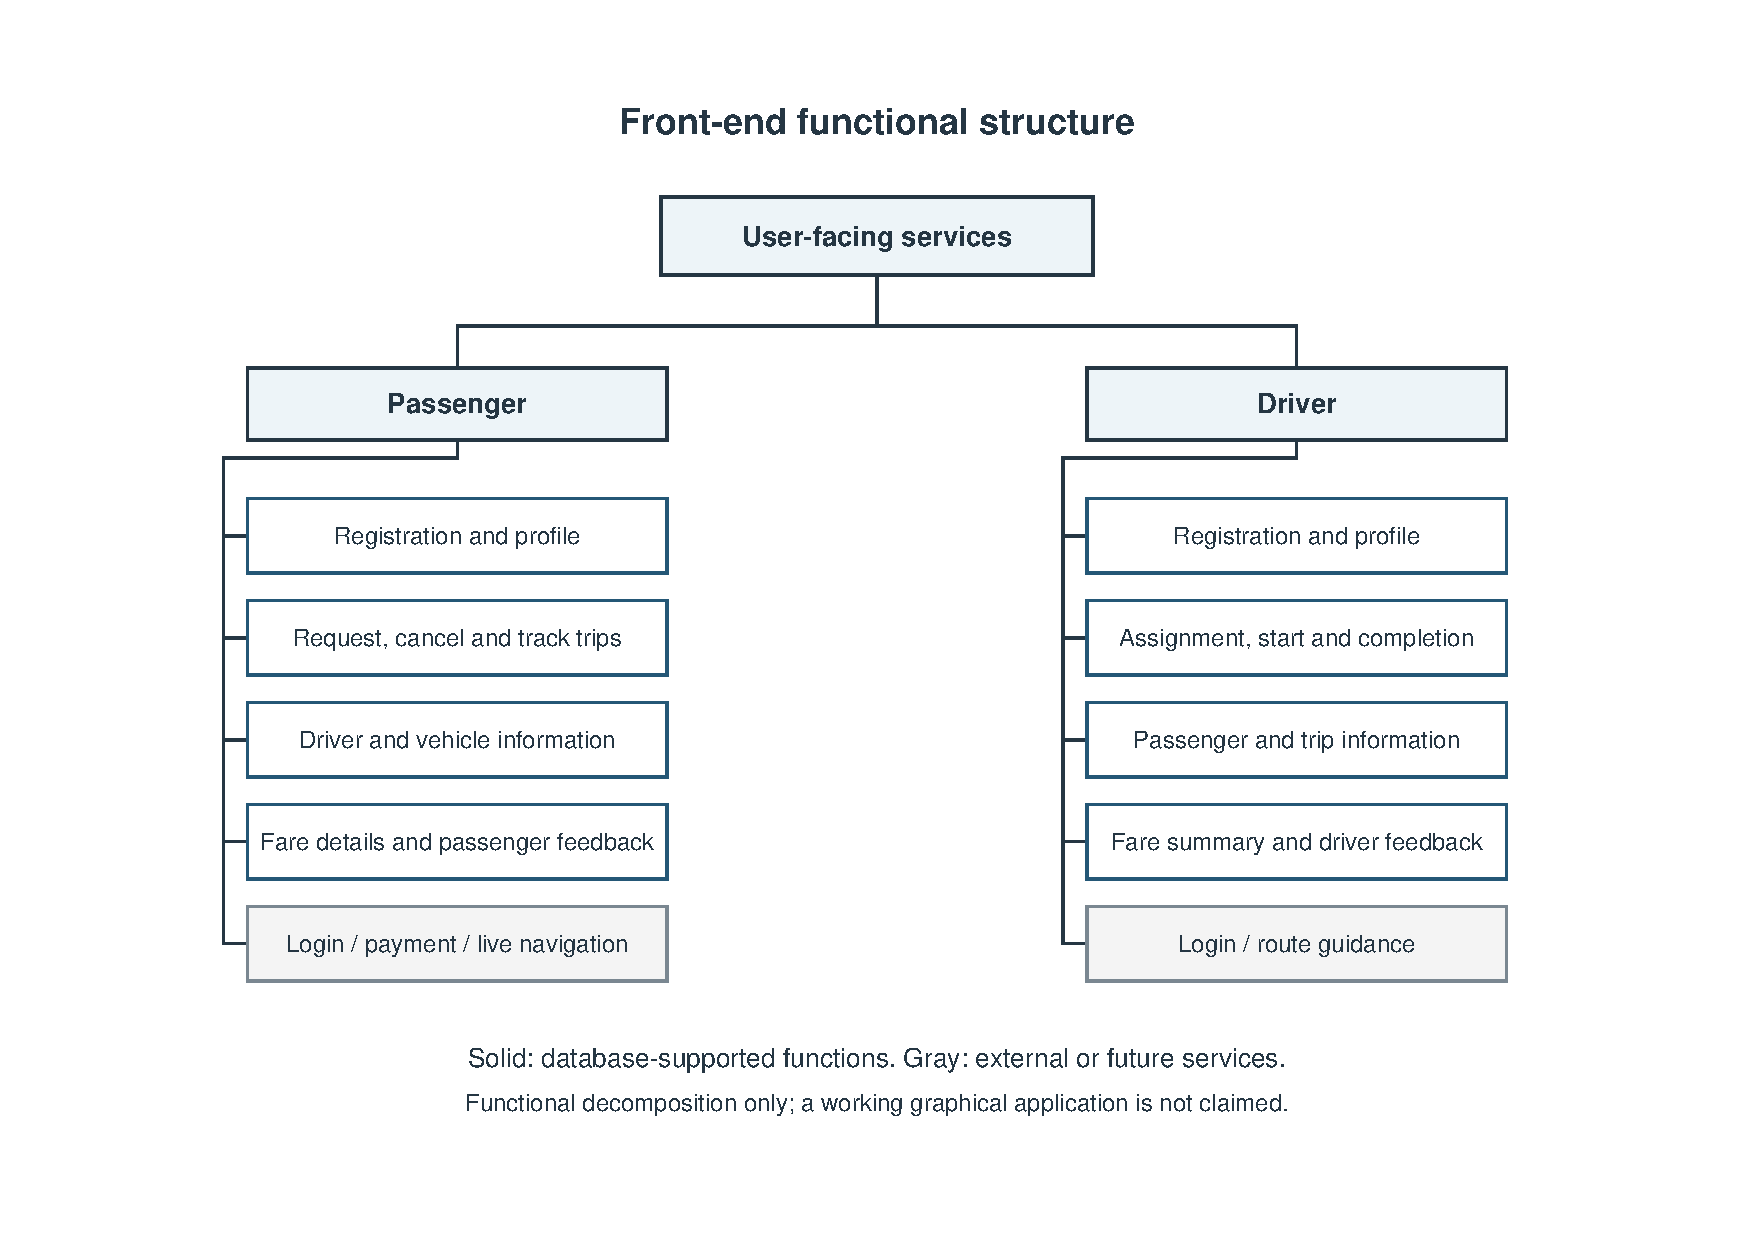
\includepdf[pages=1,fitpaper=true,pagecommand={\thispagestyle{empty}}]{figures/01_frontend.pdf}
\clearpage
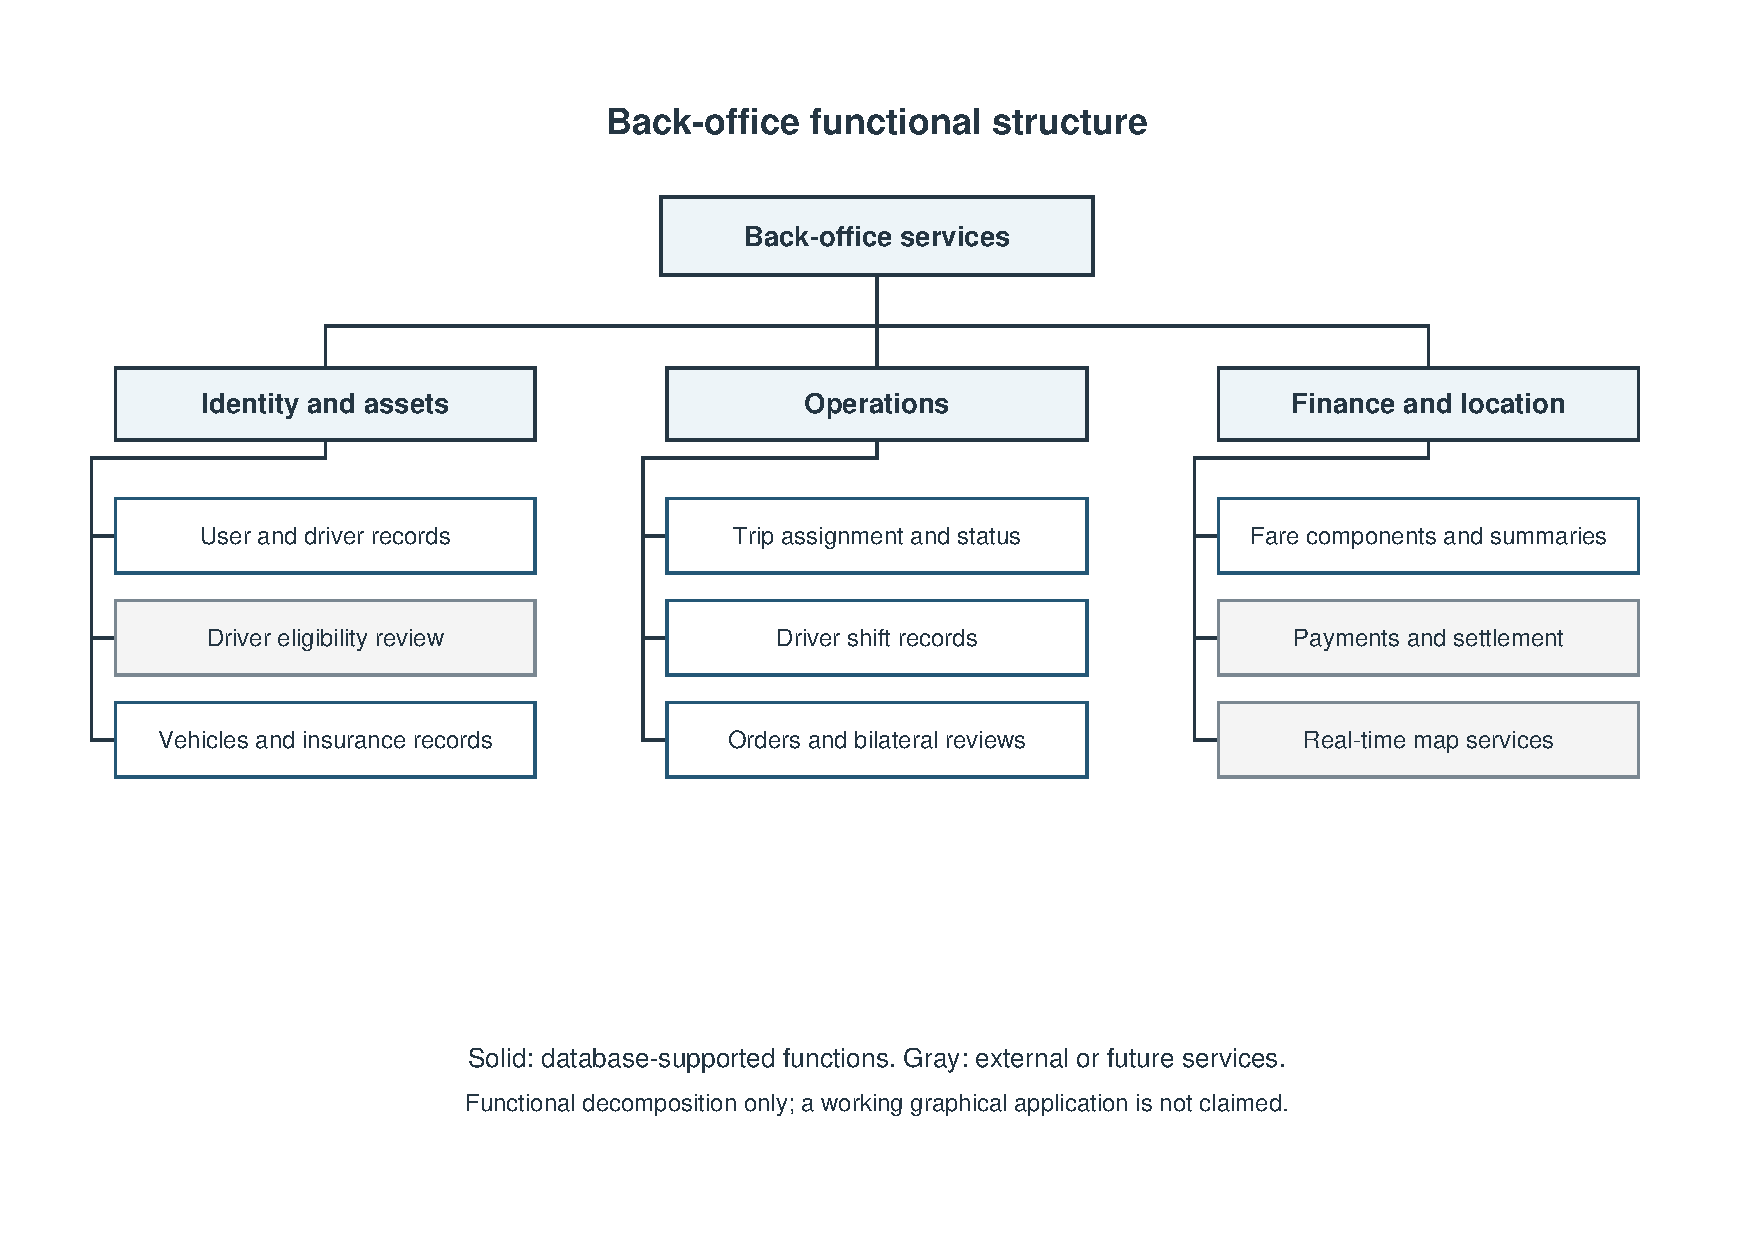
\includepdf[pages=1,fitpaper=true,pagecommand={\thispagestyle{empty}}]{figures/02_backend.pdf}

\clearpage
\section{概念设计}
\subsection{完整 ER/EER 模型}
后面的完整大图采用 LN3、LN4 的符号：矩形表示实体，椭圆表示属性，下划线表示标识符，菱形表示联系；基数用圆圈、竖线及乌鸦脚表达。DriverShift、Review、Surcharge 的身份依赖其所有者，使用双矩形；双菱形明确表示识别联系。LN3 同时说明课程并不强制区分普通联系和识别联系的菱形样式。

两个特化圆分别用 o 表示用户角色可重叠，用 d 表示行程结果互斥。父实体到特化圆的单线表示部分特化。子类继承父实体标识符，不额外重复画成椭圆。shift\_\allowbreak{}start 使用虚线下划线表示局部标识符，轮班通过司机和开始时间共同识别。评价和附加费每单最多一条，因此不需要另一个局部标识符。

图中显示全部非继承的概念属性。关系转换阶段引入的外键列在后面的关系图展示，避免在概念层重复画作普通属性。InsurancePolicy 有独立的全局唯一编号，不作为弱实体。没有连接圆点的线条交叉不表示新增联系。

\par\begingroup\small\noindent
\begin{tabularx}{\linewidth}{YY}
\toprule
符号 & 含义\\\midrule
矩形／双矩形 & 普通实体／身份依赖型实体\\
椭圆／下划线 & 属性／实体标识符\\
虚线下划线 & 所有者范围内的局部标识符\\
菱形／双菱形 & 联系／识别联系\\
圆圈加竖线；双竖线 & 零或一个；恰好一个\\
圆圈加乌鸦脚 & 零至多个\\
圆内 o／d & 重叠／互斥特化\\
父实体单线连接 & 部分特化\\
\bottomrule
\end{tabularx}
\par\endgroup
\clearpage
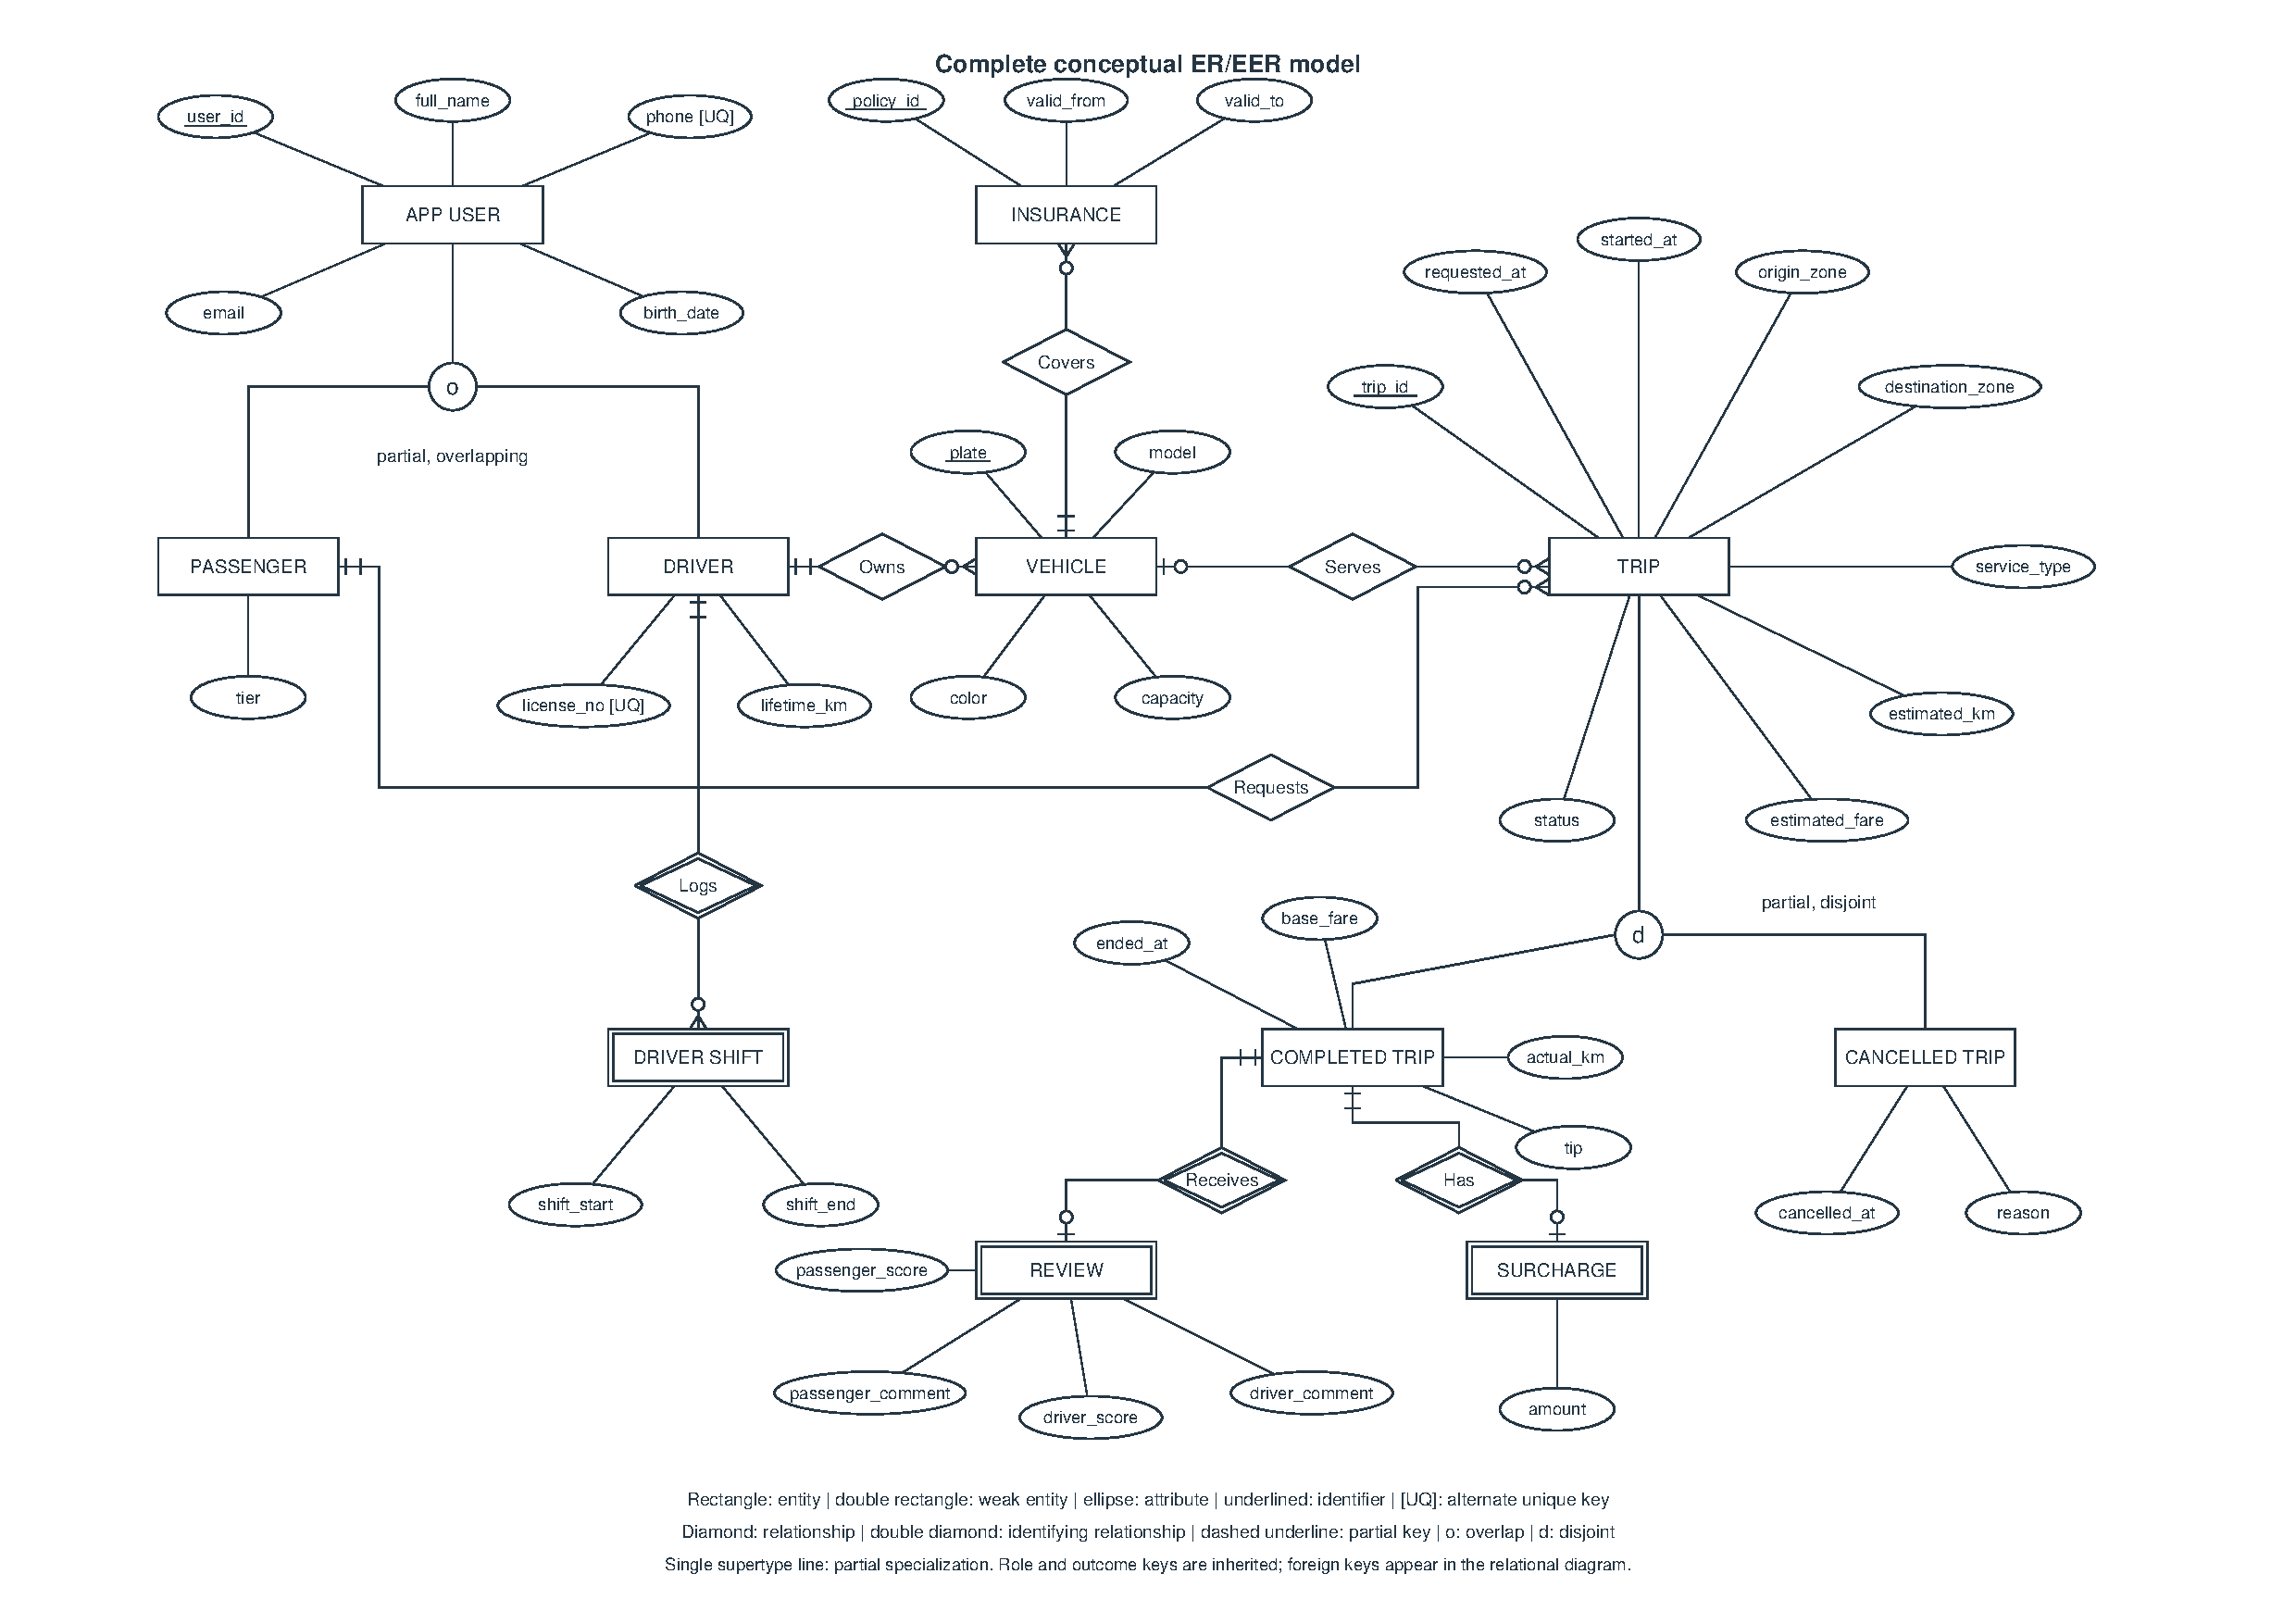
\includepdf[pages=1,fitpaper=true,pagecommand={\thispagestyle{empty}}]{figures/03_chen_eer.pdf}

\subsection{联系、参与约束与生命周期}
下表按 A → B 阅读：第二列表示一个 A 可以关联多少个 B；第三列表示一个 B 必须或可以关联多少个 A。下限为 0 表示可选参与，下限为 1 表示必选参与。完成与取消详情还必须满足下文的互斥和状态规则。

司机与行程的联系可通过车辆推导，因此不重复保存。例如 DEMO001 在观察期内归属司机 1，则使用 DEMO001 的行程对应司机 1。司机拥有多辆车时，也能明确知道每单实际使用哪一辆。

设计自然包含一对多和可选一对一联系，没有为了展示某个符号强行加入多对多联系。如果后续允许司机和车辆随时间更换对应关系，就需要新增分配历史实体，并修改当前的固定归属假设。

\par\begingroup\small\noindent
\begin{tabularx}{\linewidth}{p{4.3cm}p{1.3cm}p{1.3cm}X}
\toprule
A → B & 每个 A 的 B 数 & 每个 B 的 A 数 & 规则\\\midrule
AppUser → Passenger & 0..1 & 1 & 部分、可重叠特化\\
AppUser → Driver & 0..1 & 1 & 同一人可同时拥有两种角色\\
Driver → Vehicle & 0..N & 1 & 观察期内归属固定\\
Vehicle → InsurancePolicy & 0..N & 1 & 允许多份保单及历史记录\\
Driver → DriverShift & 0..N & 1 & 开始时间为局部标识符\\
Passenger → Trip & 0..N & 1 & 每单由一个账号请求\\
Vehicle → Trip & 0..N & 0..1 & 派单后必须存在\\
Trip → CompletedTrip & 0..1 & 1 & 只表示完成结果\\
Trip → CancelledTrip & 0..1 & 1 & 只表示取消结果\\
CompletedTrip → Review & 0..1 & 1 & 一行可包含双方评分\\
CompletedTrip → Surcharge & 0..1 & 1 & 没有记录表示无附加费\\
\bottomrule
\end{tabularx}
\par\endgroup

AppUser 的特化是部分且可重叠的：一个用户可以没有角色、只有一个角色，或同时拥有乘客和司机角色。两个子类都继承用户编号，并把它同时作为主键和外键，联系方式只保存在用户表。

行程结果是部分且互斥的特化。尚未结束的行程没有终态详情；完成状态必须恰好有一条完成详情且没有取消详情；取消状态反之。实现使用状态字段作为判别属性，通过事务把状态与详情一起写入。

本版只允许在开始前取消。进入 IN\_\allowbreak{}PROGRESS 后只允许完成，紧急中止和部分服务退款不在范围内。待接单时车辆和开始时间为空；已派单时有车辆但没有开始时间；进行中和完成状态两者都有；取消状态可以保留先前分配车辆，但没有开始时间。


\begin{center}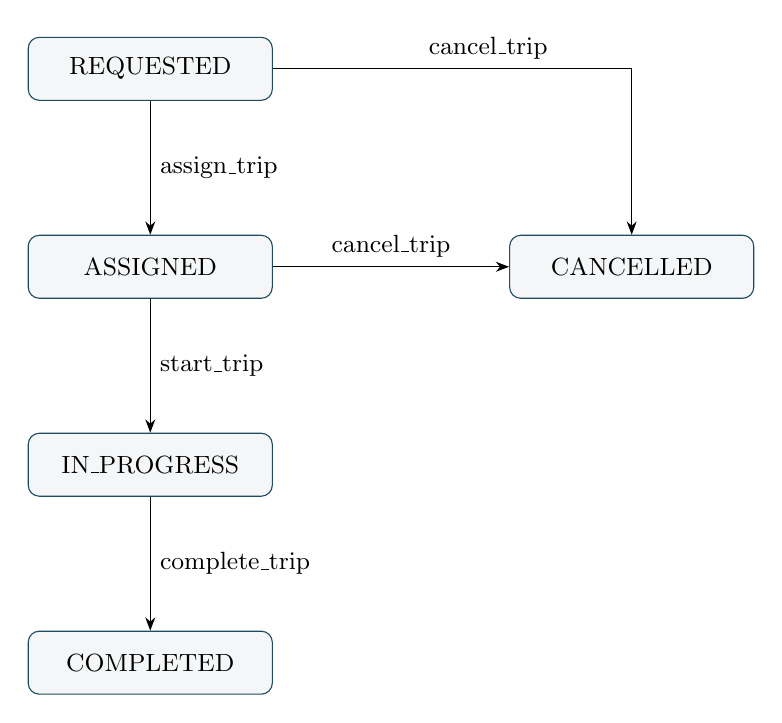
\begin{tikzpicture}[node distance=1.7cm,>=Stealth,every node/.style={font=\small},state/.style={draw=accent,rounded corners,fill=accent!5,minimum width=3.1cm,minimum height=.8cm}]
\node[state](a){REQUESTED};\node[state,below=of a](b){ASSIGNED};\node[state,below=of b](c){IN\_PROGRESS};\node[state,below=of c](d){COMPLETED};\node[state,right=3cm of b](x){CANCELLED};
\draw[->](a)--node[right]{assign\_trip}(b);\draw[->](b)--node[right]{start\_trip}(c);\draw[->](c)--node[right]{complete\_trip}(d);\draw[->](a.east)-|node[above,pos=.3]{cancel\_trip}(x.north);\draw[->](b)--node[above]{cancel\_trip}(x);
\end{tikzpicture}\end{center}
\begin{equation*}
\begin{gathered}{}[status=COMPLETED]\iff[\exists!\ CompletedTrip],\\
[status=CANCELLED]\iff[\exists!\ CancelledTrip].\end{gathered}
\end{equation*}
\clearpage
\section{关系映射与逐步规范化}
\begingroup\setlength{\parskip}{4pt}\renewcommand{\arraystretch}{1.1}\lstset{aboveskip=5pt,belowskip=5pt}
\subsection{从 ER/EER 图到初始关系模式}
本章把设计过程显式展开：先把实体和联系转换为关系，写出初始关系模式；再检查 1NF，消除部分依赖以达到 2NF，消除传递依赖以达到 3NF，最后检查所有决定因素是否满足 BCNF。每一步都明确哪些表改变、哪些表无需改变。

下面的初始模式是为说明推导而重建的设计工作稿，不代表这些中间表已经在 MySQL 执行过，也不声称逐字复制自历史文件。实际数据库只实现最终模式。工作稿在 Trip0 中同时保留车辆与所分配的司机，以对应原设计中的司机到行程联系，其余实体映射保持不变。2NF 一节另设明确标注的反例，解释司机描述属性为什么应保留在轮班关系之外；这个反例并不是新增的项目表。

\par\begingroup\small\noindent
\begin{tabularx}{\linewidth}{p{3.3cm}X}
\toprule
图中构造 & 初始关系转换\\\midrule
普通实体与属性 & 每个实体映射为一个关系，原子属性成为列；用户、司机、车辆和保单保留各自标识符。\\
用户角色特化 & 乘客与司机继承用户键作为主外键；重叠角色不重复保存公共联系方式。\\
拥有、请求、承保、服务联系 & 把一端的键放到多端：车辆保存司机编号，行程保存乘客编号和可空车牌，保险保存车牌。\\
识别联系 & 轮班使用（司机编号，开始时间）；评价与附加费继承完成行程键。\\
行程结果特化 & 完成与取消子类继承行程键；互斥及状态一致性另外用完整性规则保证。\\
\bottomrule
\end{tabularx}
\par\endgroup
例如，若先逐个联系落表，Owns(driver\_\allowbreak{}id, plate) 因为一辆车只有一名所有者而以 plate 为键；把 driver\_\allowbreak{}id 并入 Vehicle 即可吸收该联系。Requests(passenger\_\allowbreak{}id, trip\_\allowbreak{}id) 把乘客键放入 Trip；Covers(plate, policy\_\allowbreak{}id) 把车牌放入保险表；Serves(plate, trip\_\allowbreak{}id) 对应可空的 Trip.plate。这些是依据基数完成的映射选择，不是独立的规范化步骤。本范围没有需要额外桥接表的多对多联系。

\clearpage
\subsubsection*{初始模式 S0：规范化前的关系清单}
\begingroup\small\renewcommand{\arraystretch}{1.12}\begin{longtable}{p{3.1cm}p{12.1cm}}\toprule
初始关系 & 属性与候选键\\\midrule\endhead
app\_\allowbreak{}user & user\_\allowbreak{}id, full\_\allowbreak{}name, phone, email, birth\_\allowbreak{}date; 候选键：user\_\allowbreak{}id; 备用键： phone\\[4pt]
passenger & passenger\_\allowbreak{}id, tier; 候选键：passenger\_\allowbreak{}id\\[4pt]
driver & driver\_\allowbreak{}id, license\_\allowbreak{}no, lifetime\_\allowbreak{}km; 候选键：driver\_\allowbreak{}id; 备用键： license\_\allowbreak{}no\\[4pt]
vehicle & plate, driver\_\allowbreak{}id, model, color, capacity; 候选键：plate\\[4pt]
insurance\_\allowbreak{}policy & policy\_\allowbreak{}id, plate, valid\_\allowbreak{}from, valid\_\allowbreak{}to; 候选键：policy\_\allowbreak{}id\\[4pt]
driver\_\allowbreak{}shift & driver\_\allowbreak{}id, shift\_\allowbreak{}start, shift\_\allowbreak{}end; 候选键：(driver\_\allowbreak{}id, shift\_\allowbreak{}start)\\[4pt]
Trip0 & trip\_\allowbreak{}id, passenger\_\allowbreak{}id, plate, requested\_\allowbreak{}at, started\_\allowbreak{}at, origin\_\allowbreak{}zone, destination\_\allowbreak{}zone, service\_\allowbreak{}type, estimated\_\allowbreak{}km, estimated\_\allowbreak{}fare, status, driver\_\allowbreak{}id; 候选键：trip\_\allowbreak{}id\\[4pt]
completed\_\allowbreak{}trip & trip\_\allowbreak{}id, ended\_\allowbreak{}at, base\_\allowbreak{}fare, tip, actual\_\allowbreak{}km; 候选键：trip\_\allowbreak{}id\\[4pt]
cancelled\_\allowbreak{}trip & trip\_\allowbreak{}id, cancelled\_\allowbreak{}at, reason; 候选键：trip\_\allowbreak{}id\\[4pt]
review & trip\_\allowbreak{}id, passenger\_\allowbreak{}score, passenger\_\allowbreak{}comment, driver\_\allowbreak{}score, driver\_\allowbreak{}comment; 候选键：trip\_\allowbreak{}id\\[4pt]
surcharge & trip\_\allowbreak{}id, amount; 候选键：trip\_\allowbreak{}id\\[4pt]\bottomrule\end{longtable}\endgroup
DriverShift 仅保留司机键和轮班时间戳，司机描述属性留在 Driver 中。Trip0.driver\_\allowbreak{}id 表示所派车辆对应的司机，尚未分配车辆时为空。其余关系已经采用最终实体映射的属性和标识符，因此范式检查能够区分真正需要的修改与已经满足条件的关系。

\subsection{第一范式：原子值与正确的键}
1NF 要求每个属性值属于其原子值域，不能包含重复组。S0 满足这一检查：每行对应一个用户、车辆、保单、轮班或行程；phone 是一个登记电话号码；时间戳是单个 DATETIME 值。一个司机有两辆车时用两条 Vehicle 记录表示，而不是把两个车牌拼成一个字符串；多次轮班同样用多行表示。

因此 S1 = S0，无需为了声称“完成 1NF 转换”而强行拆表。轮班标识符的修正属于另一个键设计问题：同一司机一天有两班时，即便把 driver\_\allowbreak{}id 与日期组合也无法唯一标识。因此从初始映射起就采用实际开始时间。

\par\begingroup\small\noindent
\begin{tabularx}{\linewidth}{YYY}
\toprule
driver\_\allowbreak{}id & shift\_\allowbreak{}start & shift\_\allowbreak{}end\\\midrule
1 & 2026-10-01 06:00:00 & 2026-10-01 13:00:00\\
1 & 2026-10-01 14:00:00 & 2026-10-01 23:00:00\\
\bottomrule
\end{tabularx}
\par\endgroup
这两条记录来自实际运行的样例数据，司机和日历日期相同，但 shift\_\allowbreak{}start 不同。原子性与唯一性是相关但不同的设计检查；单纯修正一个不充分的键，不等于进行了 1NF 分解。

\subsection{第二范式：检查复合键依赖}
2NF 要求关系满足 1NF，且每个非主属性都完全依赖每个候选键。DriverShift 是 S1 中唯一具有复合候选键的关系，键为（driver\_\allowbreak{}id, shift\_\allowbreak{}start），唯一非主属性是 shift\_\allowbreak{}end。一个司机可以有多个轮班，不同司机也可能在同一时间开始工作，因此任一键分量都不能单独决定 shift\_\allowbreak{}end，只有完整组合能够决定。

S1 中其他关系的候选键均为单属性键。在所声明的依赖下，不存在对键的非空真子集的部分依赖。因此 S2 = S1，映射后的模式已经满足 2NF。检查通过后保持关系不变，同样是规范化过程的一部分，并不代表遗漏了转换步骤。

\begin{lstlisting}
DriverShift(driver_id, shift_start, shift_end)
Candidate key: (driver_id, shift_start)
(driver_id, shift_start) -> shift_end
Neither driver_id nor shift_start alone determines shift_end.
Decision: retain DriverShift unchanged in S2.
\end{lstlisting}
\subsubsection*{反例：什么设计会破坏第二范式？}
作为对比，假设为了方便在每条轮班记录中复制 Driver 的 license\_\allowbreak{}no 和 lifetime\_\allowbreak{}km，得到 ShiftWide。它是把现有样例记录连接起来的说明性工作表，并不是实际初始模式，也不是已实现的表。由于 license\_\allowbreak{}no 非空且唯一，这个反例的候选键将是（driver\_\allowbreak{}id, shift\_\allowbreak{}start）和（license\_\allowbreak{}no, shift\_\allowbreak{}start）。

在 ShiftWide 中，非主属性 lifetime\_\allowbreak{}km 分别只依赖 driver\_\allowbreak{}id 或 license\_\allowbreak{}no，而它们都是候选键的真子集，因此这个反例违反 2NF。license\_\allowbreak{}no 自身属于备用候选键，是主属性；判定违反 2NF 的关键是非主属性累计里程的部分依赖。

\begin{lstlisting}
Counterexample only:
ShiftWide(driver_id, shift_start, shift_end, license_no, lifetime_km)
driver_id -> license_no, lifetime_km
license_no -> driver_id, lifetime_km

Its correction would be:
Driver(driver_id, license_no, lifetime_km)
DriverShift(driver_id, shift_start, shift_end)
These are already the two relations in the mapped schema.
\end{lstlisting}
\par\begingroup\small\noindent
\begin{tabularx}{\linewidth}{YYYY}
\toprule
driver\_\allowbreak{}id & shift\_\allowbreak{}start & license\_\allowbreak{}no & lifetime\_\allowbreak{}km\\\midrule
1 & 2026-10-01 06:00:00 & DEMO-LIC-001 & 1125.00\\
1 & 2026-10-01 14:00:00 & DEMO-LIC-001 & 1125.00\\
\bottomrule
\end{tabularx}
\par\endgroup
两条重建的 ShiftWide 记录重复保存同一份登记里程，更正该值就需要更新多条轮班记录。将 Driver 与 DriverShift 分离，可以避免这种异常，并允许司机在尚未登记任何轮班时独立存在。

该示例分解无损，因为两个关系的交集 driver\_\allowbreak{}id 决定 Driver 的所有属性；按 driver\_\allowbreak{}id 连接投影可以还原原始轮班行。列出的每个依赖都能在某个分解后的关系中检查，因此保持了依赖集。最终模式本来就包含这种分离及指向所有者的外键，无需增加物理表，也不需要人为制造一次 2NF 拆分。

\subsection{第三范式、BCNF 与最终模式}
对每个非平凡依赖 X → A，3NF 要求 X 是超键，或者 A 是主属性。在 Trip0 已派车的记录中，trip\_\allowbreak{}id 决定 plate，而固定车辆归属使 plate → driver\_\allowbreak{}id 成立。同一车辆可以服务多个行程，所以 plate 不是 Trip0 的超键；driver\_\allowbreak{}id 也不是主属性。因此该依赖违反 3NF，尽管 Trip0 已经通过 2NF 检查。

\begin{lstlisting}
Trip0(trip_id, passenger_id, plate, ..., status, driver_id)
trip_id -> plate
plate -> driver_id
Therefore: trip_id -> plate -> driver_id

Project into:
Trip(trip_id, passenger_id, plate, ..., status)
VehicleOwner(plate, driver_id)

VehicleOwner is already represented inside:
Vehicle(plate, driver_id, model, color, capacity)
\end{lstlisting}
从 Trip0 删除 driver\_\allowbreak{}id，改由已有 Vehicle 表确定司机。例如实际样例的行程 1 使用 DEMO001，而 Vehicle 指明 DEMO001 对应司机 1。若重复保存的 Trip0.driver\_\allowbreak{}id 写成 2，就与车辆记录矛盾；最终模式不再允许存储这份矛盾的重复值。派单过程仍接受司机和车牌两个参数，并检查是否匹配。

对已派车行程，两个投影的交集 {plate} 决定 VehicleOwner，因此分解无损。trip\_\allowbreak{}id → plate 留在 Trip，plate → driver\_\allowbreak{}id 留在 Vehicle，它们的传递推论仍被设计保留。这个概念层证明针对车辆已存在的分配记录。未派车请求尚无车辆归属联系，在 SQL 中用 plate 为 NULL 表示；LEFT JOIN 保留这些请求，并返回空的派生司机。不能声称 INNER JOIN 也能保留未派车记录，也不能把经典的无 NULL 分解证明原样套到这些行上。

BCNF 进一步要求每个非平凡决定因素都是超键，即便被决定属性是主属性也一样。Driver 的 driver\_\allowbreak{}id 与 license\_\allowbreak{}no 都是候选键，因此满足该条件；AppUser 的 user\_\allowbreak{}id 与 phone 同理。DriverShift 唯一声明的非平凡决定因素是完整的（driver\_\allowbreak{}id, shift\_\allowbreak{}start）。其余最终关系在本项目假设下只有候选键决定的依赖。因此 S3 无需继续拆分即可达到 BCNF。下表逐一核对最终关系。

\par\begingroup\small\noindent
\begin{tabularx}{\linewidth}{p{3.0cm}p{4.0cm}X}
\toprule
关系 & 候选键 & 函数依赖\\\midrule
app\_\allowbreak{}user & user\_\allowbreak{}id; phone & 任一候选键 → 其余全部属性\\
passenger & passenger\_\allowbreak{}id & passenger\_\allowbreak{}id → tier\\
driver & driver\_\allowbreak{}id; license\_\allowbreak{}no & 任一候选键 → 其余全部属性\\
vehicle & plate & plate → driver\_\allowbreak{}id, model, color, capacity\\
insurance\_\allowbreak{}policy & policy\_\allowbreak{}id & policy\_\allowbreak{}id → plate, valid\_\allowbreak{}from, valid\_\allowbreak{}to\\
driver\_\allowbreak{}shift & (driver\_\allowbreak{}id, shift\_\allowbreak{}start) & 复合键 → shift\_\allowbreak{}end\\
trip & trip\_\allowbreak{}id & trip\_\allowbreak{}id → 其余全部属性\\
completed\_\allowbreak{}trip & trip\_\allowbreak{}id & trip\_\allowbreak{}id → ended\_\allowbreak{}at, base\_\allowbreak{}fare, tip, actual\_\allowbreak{}km\\
cancelled\_\allowbreak{}trip & trip\_\allowbreak{}id & trip\_\allowbreak{}id → cancelled\_\allowbreak{}at, reason\\
review & trip\_\allowbreak{}id & trip\_\allowbreak{}id → 双方评分和评论\\
surcharge & trip\_\allowbreak{}id & trip\_\allowbreak{}id → amount\\
\bottomrule
\end{tabularx}
\par\endgroup

这里没有额外声明 model → capacity 或距离 → 费用等依赖。容量按每辆车记录；费用还包含不能仅由距离确定的组成部分。范式结论来自已声明的业务语义，不能仅凭少量样例数据证明真实世界的一切函数依赖。

另外，有些改动不属于范式分解：分开完成与取消详情是在表达互斥结果；附加费单独保存是在表达可选的一对一详情，把 amount 并入 CompletedTrip 本身并不违反 BCNF；评价采用 trip\_\allowbreak{}id 为键，是为了每单最多一条双向反馈，而独立 review\_\allowbreak{}id 加 UNIQUE(trip\_\allowbreak{}id) 也可以满足范式。不能把这些选择写成从 2NF 到 3NF 必须执行的拆分。

\par\begingroup\small\noindent
\begin{tabularx}{\linewidth}{p{2.5cm}p{6.2cm}X}
\toprule
阶段 & 检查与处理 & 结果\\\midrule
S0 → S1 & 原子值；正确的轮班标识符 & 已满足 1NF，不拆表\\
S1 → S2 & 检查 DriverShift 的复合键 & 已满足 2NF，无需拆分\\
S2 → S3 & 消除 Trip0 中车牌到司机的传递依赖 & Trip + 已有 Vehicle，达到 3NF\\
S3 → BCNF & 检查所有非平凡决定因素 & 无需继续分解，最终 11 张表\\
\bottomrule
\end{tabularx}
\par\endgroup
下面的最终关系图展示全部 11 张运营表及实现字段。PK、FK、UQ 分别表示主键、外键和备用唯一键，问号表示字段可空。图中的字段由实际执行的 MySQL 数据字典生成，与后续 SQL 实现一致。

\clearpage
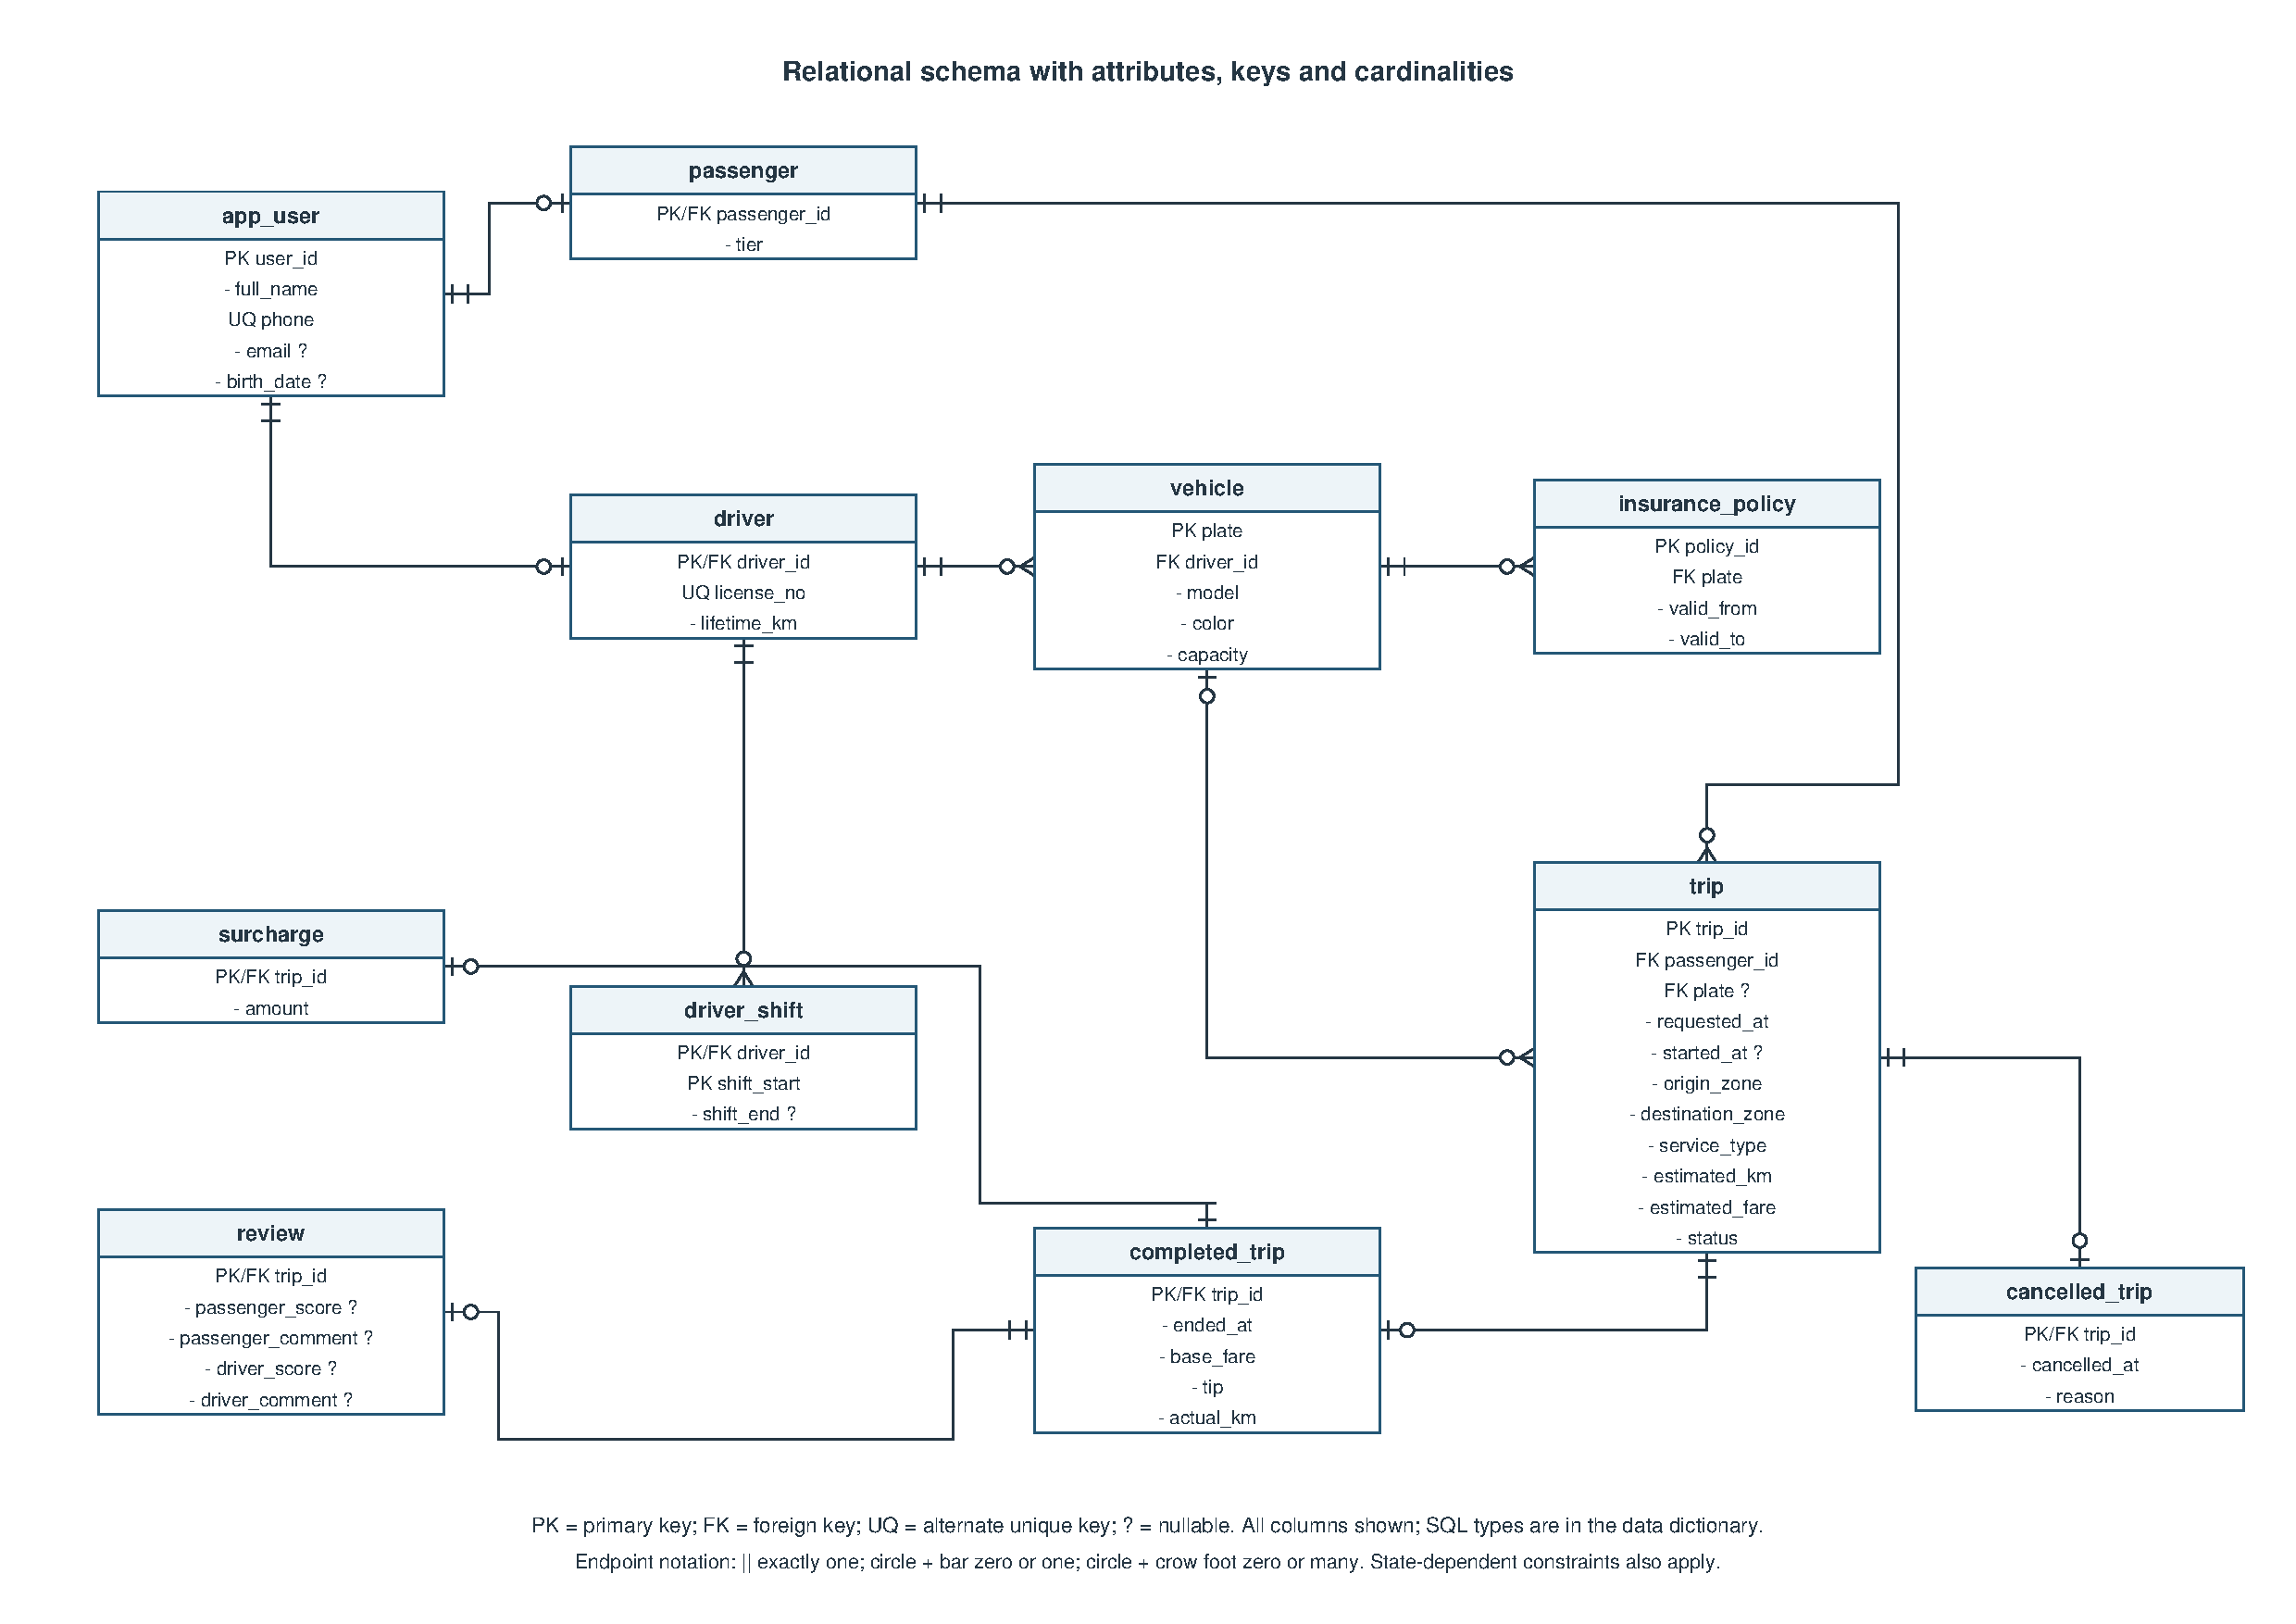
\includepdf[pages=1,fitpaper=true,pagecommand={\thispagestyle{empty}}]{figures/04_relational.pdf}
\endgroup
\clearpage
\section{数据库实现与验证}
\subsection{物理表、约束与建表 SQL}
实际执行引擎为 MySQL 8.4.13，所有运营表使用 InnoDB。主键和唯一约束保护实体标识，外键保护引用，CHECK 检查本行的值域和时间顺序。删除引用对象时采用默认限制策略，不从用户向历史行程进行大范围级联删除。

应用角色可以创建身份和登记记录，只能插入允许的下单字段，可以提交或修改评价、读取结果，并调用生命周期过程。它不能直接修改 Trip.status，也不能直接写入结果子表。过程通过定义者权限完成受控操作。测试用临时账号在验证后删除，交付不提供无密码生产账号。

保护触发器检查完成记录的父状态和结束时间、取消记录的父状态和取消时间，并禁止车辆归属变更。跨表一致性不能全部依靠本行 CHECK，因此通过事务过程把状态和详情作为一个整体写入。拥有直接写权限的管理员仍可能绕过流程；一致性保证针对声明的应用接口和角色。

索引包括用于乘客历史查询的 (passenger\_\allowbreak{}id, requested\_\allowbreak{}at) 和用于运营筛选的 (status, requested\_\allowbreak{}at)。主外键索引支持连接。保存的 EXPLAIN 反映小样本上的实际优化器选择，不据此声称达到生产性能。本次乘客历史查询实际使用 ix\_\allowbreak{}trip\_\allowbreak{}passenger\_\allowbreak{}time 的 range 访问，估计扫描 3 行，Extra 为 Using index condition。

\begin{lstlisting}
CREATE VIEW trip_service AS
SELECT t.*, v.driver_id
FROM trip t LEFT JOIN vehicle v ON v.plate=t.plate;

-- A booking cannot directly choose status or completion detail
-- when inserted through the application role.
GRANT INSERT (trip_id, passenger_id, requested_at,
 origin_zone, destination_zone, service_type,
 estimated_km, estimated_fare)
ON ride_hailing.trip TO 'ride_hailing_app';
\end{lstlisting}

下面直接列出实际执行的全部 11 张运营表的建表 SQL，包含建库语句、主键和备用键、外键、值域约束及索引。创建顺序遵循先父表后子表，不需要关闭外键检查。

所有表采用支持事务的 InnoDB。如果 schema 已存在，脚本会明确报错，不会为了运行演示而悄悄删除数据。过程和触发器的完整定义仍在配套 SQL 文件中，生命周期章节解释其作用。

\lstinputlisting[language=SQL,basicstyle=\ttfamily\footnotesize]{sql/01_schema.sql}
\subsection{数据装载与 SQL 实际演示}
生成器使用固定随机种子 20261118，生成 2026 年 10 月 1 日至 20 日期间请求的 200 条行程。各状态数量预先设定，再打乱分布到整个期间。时间使用上海本地民用时间，以 DATETIME 保存，本单地区示例不处理时区转换。

数据包含一个双角色用户、一个尚无角色的注册用户、部分司机拥有多辆车，以及每位司机每天两次轮班。完成行程覆盖可选打赏、附加费、单边和双边评价。取消可以发生在派单前或派单后；开放状态用于验证可选关联。

姓名、联系方式、驾驶证和车牌均为虚构，邮箱使用 example.invalid。状态比例和费用来自生成规则，不是实测业务表现。司机 lifetime\_\allowbreak{}km 是登记快照，不由本批行程自动累加。

复现流程依次创建新 schema、加载过程、生成并通过生命周期接口导入数据、建立分析快照、创建应用角色和运行验证。测试使用保留编号，发布查询结果前清除这些临时记录。随机种子、实际行数、SQL 及查询输出一并保留。

\par\begingroup\small\noindent
\begin{tabularx}{\linewidth}{YY}
\toprule
运营表 & 行数\\\midrule
app\_\allowbreak{}user & 34\\
passenger & 26\\
driver & 8\\
vehicle & 12\\
insurance\_\allowbreak{}policy & 12\\
driver\_\allowbreak{}shift & 320\\
trip & 200\\
completed\_\allowbreak{}trip & 130\\
cancelled\_\allowbreak{}trip & 30\\
review & 98\\
surcharge & 52\\
\bottomrule
\end{tabularx}
\par\endgroup

SHOW TABLES 展示建库后实际存在的对象：11 张运营表、4 张 dw\_\allowbreak{} 分析表和 2 个视图。DESCRIBE trip 进一步展示实际字段结构。下方选取 Field、Type、Null、Key 四列展示，完整原始输出在证据文件中。

\noindent\begin{minipage}[t]{.29\linewidth}\vspace{0pt}\par\noindent\begin{minipage}{\linewidth}\setlength{\parskip}{0pt}\renewcommand{\arraystretch}{1.08}\titlespacing*{\subsection}{0pt}{7pt}{4pt}\lstset{aboveskip=4pt,belowskip=4pt}
\subsection*{show\_\allowbreak{}tables}
\begin{lstlisting}
SHOW TABLES;
\end{lstlisting}
\par\begingroup\small\noindent
\begin{tabularx}{\linewidth}{Y}
\toprule
Tables\_\allowbreak{}in\_\allowbreak{}ride\_\allowbreak{}hailing\\\midrule
app\_\allowbreak{}user\\
cancelled\_\allowbreak{}trip\\
completed\_\allowbreak{}trip\\
driver\\
driver\_\allowbreak{}shift\\
dw\_\allowbreak{}date\\
dw\_\allowbreak{}driver\\
dw\_\allowbreak{}trip\_\allowbreak{}fact\\
dw\_\allowbreak{}vehicle\\
insurance\_\allowbreak{}policy\\
passenger\\
review\\
surcharge\\
trip\\
trip\_\allowbreak{}financials\\
trip\_\allowbreak{}service\\
vehicle\\
\bottomrule
\end{tabularx}
\par\endgroup
\end{minipage}\par\vspace{5pt}
\end{minipage}\hfill\begin{minipage}[t]{.68\linewidth}\vspace{0pt}\par\noindent\begin{minipage}{\linewidth}\setlength{\parskip}{0pt}\renewcommand{\arraystretch}{1.08}\titlespacing*{\subsection}{0pt}{7pt}{4pt}\lstset{aboveskip=4pt,belowskip=4pt}
\subsection*{describe\_\allowbreak{}trip}
\begin{lstlisting}
DESCRIBE trip;
\end{lstlisting}
\par\begingroup\small\noindent
\begin{tabularx}{\linewidth}{YYYY}
\toprule
Field & Type & 可为空 & 键标记\\\midrule
trip\_\allowbreak{}id & int & NO & PRI\\
passenger\_\allowbreak{}id & int & NO & MUL\\
plate & varchar(12) & YES & MUL\\
requested\_\allowbreak{}at & datetime & NO & \\
started\_\allowbreak{}at & datetime & YES & \\
origin\_\allowbreak{}zone & varchar(30) & NO & \\
destination\_\allowbreak{}zone & varchar(30) & NO & \\
service\_\allowbreak{}type & varchar(12) & NO & \\
estimated\_\allowbreak{}km & decimal(8,2) & NO & \\
estimated\_\allowbreak{}fare & decimal(10,2) & NO & \\
status & varchar(12) & NO & MUL\\
\bottomrule
\end{tabularx}
\par\endgroup
\end{minipage}\par\vspace{5pt}
\end{minipage}
\subsubsection*{用户与角色的数据展示}
以下按键排序的 SELECT 展示实际插入数据。用户 1 同时出现在乘客表和司机表中，体现可重叠特化。用户样例选取身份字段展示，完整字段定义见数据字典。

\par\noindent\begin{minipage}{\linewidth}\setlength{\parskip}{0pt}\renewcommand{\arraystretch}{1.08}\titlespacing*{\subsection}{0pt}{7pt}{4pt}\lstset{aboveskip=4pt,belowskip=4pt}
\subsection*{app\_\allowbreak{}user}
\begin{lstlisting}
SELECT user_id,full_name,phone
FROM app_user
ORDER BY user_id LIMIT 3;
\end{lstlisting}
\par\begingroup\small\noindent
\begin{tabularx}{\linewidth}{YYY}
\toprule
user\_\allowbreak{}id & full\_\allowbreak{}name & phone\\\midrule
1 & Demo User 1 & +860000000001\\
2 & Demo User 2 & +860000000002\\
3 & Demo User 3 & +860000000003\\
\bottomrule
\end{tabularx}
\par\endgroup
\end{minipage}\par\vspace{5pt}
\par\noindent\begin{minipage}{\linewidth}\setlength{\parskip}{0pt}\renewcommand{\arraystretch}{1.08}\titlespacing*{\subsection}{0pt}{7pt}{4pt}\lstset{aboveskip=4pt,belowskip=4pt}
\subsection*{passenger}
\begin{lstlisting}
SELECT *
FROM passenger
ORDER BY passenger_id LIMIT 3;
\end{lstlisting}
\par\begingroup\small\noindent
\begin{tabularx}{\linewidth}{YY}
\toprule
passenger\_\allowbreak{}id & tier\\\midrule
1 & PLATINUM\\
101 & STANDARD\\
102 & GOLD\\
\bottomrule
\end{tabularx}
\par\endgroup
\end{minipage}\par\vspace{5pt}
\par\noindent\begin{minipage}{\linewidth}\setlength{\parskip}{0pt}\renewcommand{\arraystretch}{1.08}\titlespacing*{\subsection}{0pt}{7pt}{4pt}\lstset{aboveskip=4pt,belowskip=4pt}
\subsection*{driver}
\begin{lstlisting}
SELECT *
FROM driver
ORDER BY driver_id LIMIT 3;
\end{lstlisting}
\par\begingroup\small\noindent
\begin{tabularx}{\linewidth}{YYY}
\toprule
driver\_\allowbreak{}id & license\_\allowbreak{}no & lifetime\_\allowbreak{}km\\\midrule
1 & DEMO-LIC-001 & 1125.00\\
2 & DEMO-LIC-002 & 1250.00\\
3 & DEMO-LIC-003 & 1375.00\\
\bottomrule
\end{tabularx}
\par\endgroup
\end{minipage}\par\vspace{5pt}

\subsubsection*{车辆保险与轮班的数据展示}
下列数据展示车辆到司机、保单到车辆的关联。轮班样例包含同一司机在同一天的两个班次，说明仅用日期不足以作为局部标识符。这些合成记录由 MySQL 实际查询返回，并非手工填写的预期结果。

\par\noindent\begin{minipage}{\linewidth}\setlength{\parskip}{0pt}\renewcommand{\arraystretch}{1.08}\titlespacing*{\subsection}{0pt}{7pt}{4pt}\lstset{aboveskip=4pt,belowskip=4pt}
\subsection*{vehicle}
\begin{lstlisting}
SELECT *
FROM vehicle
ORDER BY plate LIMIT 3;
\end{lstlisting}
\par\begingroup\small\noindent
\begin{tabularx}{\linewidth}{YYYYY}
\toprule
plate & driver\_\allowbreak{}id & model & color & capacity\\\midrule
DEMO001 & 1 & MPV & Blue & 4\\
DEMO002 & 2 & Electric & Black & 4\\
DEMO003 & 3 & Sedan & White & 6\\
\bottomrule
\end{tabularx}
\par\endgroup
\end{minipage}\par\vspace{5pt}
\par\noindent\begin{minipage}{\linewidth}\setlength{\parskip}{0pt}\renewcommand{\arraystretch}{1.08}\titlespacing*{\subsection}{0pt}{7pt}{4pt}\lstset{aboveskip=4pt,belowskip=4pt}
\subsection*{insurance\_\allowbreak{}policy}
\begin{lstlisting}
SELECT *
FROM insurance_policy
ORDER BY policy_id LIMIT 3;
\end{lstlisting}
\par\begingroup\small\noindent
\begin{tabularx}{\linewidth}{YYYY}
\toprule
policy\_\allowbreak{}id & plate & valid\_\allowbreak{}from & valid\_\allowbreak{}to\\\midrule
1 & DEMO001 & 2026-01-01 & 2026-11-10\\
2 & DEMO002 & 2026-01-01 & 2026-11-10\\
3 & DEMO003 & 2026-01-01 & 2026-11-10\\
\bottomrule
\end{tabularx}
\par\endgroup
\end{minipage}\par\vspace{5pt}
\par\noindent\begin{minipage}{\linewidth}\setlength{\parskip}{0pt}\renewcommand{\arraystretch}{1.08}\titlespacing*{\subsection}{0pt}{7pt}{4pt}\lstset{aboveskip=4pt,belowskip=4pt}
\subsection*{driver\_\allowbreak{}shift}
\begin{lstlisting}
SELECT *
FROM driver_shift
ORDER BY driver_id,shift_start LIMIT 3;
\end{lstlisting}
\par\begingroup\small\noindent
\begin{tabularx}{\linewidth}{YYY}
\toprule
driver\_\allowbreak{}id & shift\_\allowbreak{}start & shift\_\allowbreak{}end\\\midrule
1 & 2026-10-01 06:00:00 & 2026-10-01 13:00:00\\
1 & 2026-10-01 14:00:00 & 2026-10-01 23:00:00\\
1 & 2026-10-02 06:00:00 & 2026-10-02 13:00:00\\
\bottomrule
\end{tabularx}
\par\endgroup
\end{minipage}\par\vspace{5pt}

\subsubsection*{行程与结果的数据展示}
Trip 保存请求及当前状态，终态详情保存对应结果的专属属性。为便于阅读，主表样例选取编号、派车、状态和预估费用；两种结果子表使用 SELECT *。完整数据在种子 SQL 中提供。

\par\noindent\begin{minipage}{\linewidth}\setlength{\parskip}{0pt}\renewcommand{\arraystretch}{1.08}\titlespacing*{\subsection}{0pt}{7pt}{4pt}\lstset{aboveskip=4pt,belowskip=4pt}
\subsection*{trip}
\begin{lstlisting}
SELECT trip_id,passenger_id,plate,status,estimated_fare
FROM trip
ORDER BY trip_id LIMIT 6;
\end{lstlisting}
\par\begingroup\small\noindent
\begin{tabularx}{\linewidth}{YYYYY}
\toprule
trip\_\allowbreak{}id & passenger\_\allowbreak{}id & plate & status & estimated\_\allowbreak{}fare\\\midrule
1 & 1 & DEMO001 & COMPLETED & 87.17\\
2 & 118 & NULL & REQUESTED & 40.64\\
3 & 111 & DEMO003 & IN\_\allowbreak{}PROGRESS & 88.69\\
4 & 124 & DEMO004 & COMPLETED & 31.70\\
5 & 125 & DEMO005 & ASSIGNED & 20.08\\
6 & 101 & NULL & CANCELLED & 53.75\\
\bottomrule
\end{tabularx}
\par\endgroup
\end{minipage}\par\vspace{5pt}
\par\noindent\begin{minipage}{\linewidth}\setlength{\parskip}{0pt}\renewcommand{\arraystretch}{1.08}\titlespacing*{\subsection}{0pt}{7pt}{4pt}\lstset{aboveskip=4pt,belowskip=4pt}
\subsection*{completed\_\allowbreak{}trip}
\begin{lstlisting}
SELECT *
FROM completed_trip
ORDER BY trip_id LIMIT 3;
\end{lstlisting}
\par\begingroup\small\noindent
\begin{tabularx}{\linewidth}{YYYYY}
\toprule
trip\_\allowbreak{}id & ended\_\allowbreak{}at & base\_\allowbreak{}fare & tip & actual\_\allowbreak{}km\\\midrule
1 & 2026-10-01 09:36:00 & 91.52 & 0.00 & 24.38\\
4 & 2026-10-01 12:39:00 & 27.01 & 2.00 & 15.39\\
7 & 2026-10-01 15:42:00 & 74.28 & 0.00 & 14.32\\
\bottomrule
\end{tabularx}
\par\endgroup
\end{minipage}\par\vspace{5pt}
\par\noindent\begin{minipage}{\linewidth}\setlength{\parskip}{0pt}\renewcommand{\arraystretch}{1.08}\titlespacing*{\subsection}{0pt}{7pt}{4pt}\lstset{aboveskip=4pt,belowskip=4pt}
\subsection*{cancelled\_\allowbreak{}trip}
\begin{lstlisting}
SELECT *
FROM cancelled_trip
ORDER BY trip_id LIMIT 3;
\end{lstlisting}
\par\begingroup\small\noindent
\begin{tabularx}{\linewidth}{YYY}
\toprule
trip\_\allowbreak{}id & cancelled\_\allowbreak{}at & reason\\\midrule
6 & 2026-10-01 14:10:00 & Waiting time\\
14 & 2026-10-02 12:18:00 & Waiting time\\
18 & 2026-10-02 16:22:00 & Plans changed\\
\bottomrule
\end{tabularx}
\par\endgroup
\end{minipage}\par\vspace{5pt}

\subsubsection*{评价附加费及连接查询结果}
评价样例展示双方评分及缺失值，附加费表只在确有附加费时存在记录。最后的 LEFT JOIN 把行程状态、实际车辆、派生司机及总费用联系起来。开放或取消行程仍保留在结果中，由于没有完成详情，其 total\_\allowbreak{}fare 为 NULL。

\par\noindent\begin{minipage}{\linewidth}\setlength{\parskip}{0pt}\renewcommand{\arraystretch}{1.08}\titlespacing*{\subsection}{0pt}{7pt}{4pt}\lstset{aboveskip=4pt,belowskip=4pt}
\subsection*{review}
\begin{lstlisting}
SELECT trip_id,passenger_score,driver_score
FROM review
ORDER BY trip_id LIMIT 3;
\end{lstlisting}
\par\begingroup\small\noindent
\begin{tabularx}{\linewidth}{YYY}
\toprule
trip\_\allowbreak{}id & passenger\_\allowbreak{}score & driver\_\allowbreak{}score\\\midrule
1 & 92 & 93\\
7 & 67 & 77\\
9 & 66 & NULL\\
\bottomrule
\end{tabularx}
\par\endgroup
\end{minipage}\par\vspace{5pt}
\par\noindent\begin{minipage}{\linewidth}\setlength{\parskip}{0pt}\renewcommand{\arraystretch}{1.08}\titlespacing*{\subsection}{0pt}{7pt}{4pt}\lstset{aboveskip=4pt,belowskip=4pt}
\subsection*{surcharge}
\begin{lstlisting}
SELECT *
FROM surcharge
ORDER BY trip_id LIMIT 3;
\end{lstlisting}
\par\begingroup\small\noindent
\begin{tabularx}{\linewidth}{YY}
\toprule
trip\_\allowbreak{}id & amount\\\midrule
9 & 4.00\\
11 & 4.00\\
15 & 4.00\\
\bottomrule
\end{tabularx}
\par\endgroup
\end{minipage}\par\vspace{5pt}
\par\noindent\begin{minipage}{\linewidth}\setlength{\parskip}{0pt}\renewcommand{\arraystretch}{1.08}\titlespacing*{\subsection}{0pt}{7pt}{4pt}\lstset{aboveskip=4pt,belowskip=4pt}
\subsection*{joined\_\allowbreak{}example}
\begin{lstlisting}
SELECT t.trip_id,t.status,t.plate,v.driver_id,t.estimated_fare,f.total_fare
FROM trip t LEFT JOIN vehicle v ON v.plate=t.plate LEFT JOIN trip_financials f ON f.trip_id=t.trip_id
ORDER BY t.trip_id LIMIT 6;
\end{lstlisting}
\par\begingroup\small\noindent
\begin{tabularx}{\linewidth}{YYYYYY}
\toprule
trip\_\allowbreak{}id & status & plate & driver\_\allowbreak{}id & estimated\_\allowbreak{}fare & total\_\allowbreak{}fare\\\midrule
1 & COMPLETED & DEMO001 & 1 & 87.17 & 91.52\\
2 & REQUESTED & NULL & NULL & 40.64 & NULL\\
3 & IN\_\allowbreak{}PROGRESS & DEMO003 & 3 & 88.69 & NULL\\
4 & COMPLETED & DEMO004 & 4 & 31.70 & 29.01\\
5 & ASSIGNED & DEMO005 & 5 & 20.08 & NULL\\
6 & CANCELLED & NULL & NULL & 53.75 & NULL\\
\bottomrule
\end{tabularx}
\par\endgroup
\end{minipage}\par\vspace{5pt}

\subsubsection*{插入修改删除及实际结果}
本例使用临时用户演示三种写操作及实际结果：先插入，再修改姓名，最后删除。每一步后都查询数据库状态。最终计数为 0，临时记录不属于发布的样例数据。删除被历史记录引用的用户属于另一项负向测试，会被外键拒绝。

\par\noindent\begin{minipage}{\linewidth}\setlength{\parskip}{0pt}\renewcommand{\arraystretch}{1.08}\titlespacing*{\subsection}{0pt}{7pt}{4pt}\lstset{aboveskip=4pt,belowskip=4pt}
\subsection*{crud\_\allowbreak{}insert}
\begin{lstlisting}
INSERT INTO app_user(user_id,full_name,phone) VALUES(9998,'CRUD Demo','demo-crud-9998');
SELECT user_id,full_name,phone
FROM app_user WHERE user_id=9998;
\end{lstlisting}
\par\begingroup\small\noindent
\begin{tabularx}{\linewidth}{YYY}
\toprule
user\_\allowbreak{}id & full\_\allowbreak{}name & phone\\\midrule
9998 & CRUD Demo & demo-crud-9998\\
\bottomrule
\end{tabularx}
\par\endgroup
\end{minipage}\par\vspace{5pt}
\par\noindent\begin{minipage}{\linewidth}\setlength{\parskip}{0pt}\renewcommand{\arraystretch}{1.08}\titlespacing*{\subsection}{0pt}{7pt}{4pt}\lstset{aboveskip=4pt,belowskip=4pt}
\subsection*{crud\_\allowbreak{}update}
\begin{lstlisting}
UPDATE app_user SET full_name='CRUD Updated' WHERE user_id=9998;
SELECT user_id,full_name,phone
FROM app_user WHERE user_id=9998;
\end{lstlisting}
\par\begingroup\small\noindent
\begin{tabularx}{\linewidth}{YYY}
\toprule
user\_\allowbreak{}id & full\_\allowbreak{}name & phone\\\midrule
9998 & CRUD Updated & demo-crud-9998\\
\bottomrule
\end{tabularx}
\par\endgroup
\end{minipage}\par\vspace{5pt}
\par\noindent\begin{minipage}{\linewidth}\setlength{\parskip}{0pt}\renewcommand{\arraystretch}{1.08}\titlespacing*{\subsection}{0pt}{7pt}{4pt}\lstset{aboveskip=4pt,belowskip=4pt}
\subsection*{crud\_\allowbreak{}delete}
\begin{lstlisting}
DELETE
FROM app_user WHERE user_id=9998;
SELECT COUNT(*) AS remaining
FROM app_user WHERE user_id=9998;
\end{lstlisting}
\par\begingroup\small\noindent
\begin{tabularx}{\linewidth}{Y}
\toprule
remaining\\\midrule
0\\
\bottomrule
\end{tabularx}
\par\endgroup
\end{minipage}\par\vspace{5pt}

\subsection{事务、并发与验证}
每个生命周期过程先开始事务，用 SELECT ... FOR UPDATE 锁定目标行程，检查当前状态，执行必要写入，然后提交。异常处理器回滚并重新抛出错误。过程负责自己的事务边界，因此调用方不能在已开启的事务中调用；这里没有嵌套事务语义。

派单验证指定司机是否拥有指定车辆。开始过程要求状态为 ASSIGNED，并由 CHECK 拒绝早于下单的开始时间。完成过程先写入完成详情，再验证和写入可选附加费，最后改变主表状态。取消过程同样写详情并更新状态。行锁使同一行程的竞争操作依次执行。

回滚测试故意让完成详情先插入，再提交负附加费触发异常。正确结果应撤销前面的详情插入，且父行程仍为 IN\_\allowbreak{}PROGRESS。这验证了多步写入的原子性，而不只是入口处拒绝非法输入。

并发测试使用两个独立客户端同时完成同一进行中订单。应恰好一个成功，另一个获得锁后发现终态并被拒绝。这验证同一订单的串行化，不等于测试了多司机调度、分布式故障、吞吐量或司机重复派单预防。

\begin{lstlisting}
START TRANSACTION;
SELECT status INTO v_status
FROM trip WHERE trip_id=p_trip FOR UPDATE;
-- Require IN_PROGRESS, otherwise SIGNAL SQLSTATE '45000'.
INSERT INTO completed_trip VALUES
 (p_trip,p_end,p_base,p_tip,p_km);
-- Invalid surcharge raises an error here; handler rolls back.
IF p_extra > 0 THEN
 INSERT INTO surcharge VALUES(p_trip,p_extra);
END IF;
UPDATE trip SET status='COMPLETED' WHERE trip_id=p_trip;
COMMIT;
\end{lstlisting}

本次数据库运行记录的 32 项检查全部通过。负向测试要求出现指定 MySQL 错误类别，不会把任意失败都当成通过。覆盖身份与引用完整性、值域、时间顺序、流程规则、回滚、并发完成、应用权限及分析层核对。

成功的插入、修改和删除使用临时记录演示；删除被引用用户的尝试被拒绝。权限测试确认应用角色不能直接更新行程状态，但允许下单并调用取消过程。

下表按类型汇总，完整测试名称、通过标记及错误消息保存在 validation.json。这些检查为声明的流程和样例数据提供证据，不代表生产就绪，也没有完成崩溃恢复或穷尽安全测试。

\par\begingroup\small\noindent
\begin{tabularx}{\linewidth}{p{2.5cm}Yp{1.5cm}}
\toprule
类别 & 实际检查 & 结果\\\midrule
键与引用 & 重复编号、重复评价、无效父记录、受限删除 & 通过\\
值域 & 越界评分、空评价、负金额、姓名必填 & 通过\\
时间 & 轮班结束、开始早于请求、完成早于开始 & 通过\\
流程 & 归属固定、错误司机、互斥结果、终态限制 & 通过\\
事务 & 撤销部分写入、保留原状态、成功路径 & 通过\\
并发 & 两次完成请求中恰好一次提交 & 通过\\
权限 & 禁止直接改状态，允许授权下单和取消 & 通过\\
核对 & 200 单、状态详情一致、连接无放大、仓库行数金额一致 & 通过\\
样例覆盖 & 重叠角色、同日双轮班、增改删清理 & 通过\\
\bottomrule
\end{tabularx}
\par\endgroup

\clearpage
\section{数据使用、讨论与结论}
\subsection{运营查询与实际结果}
费用视图把每条完成行程与至多一条附加费连接。COALESCE 把不存在的可选附加费视作 0，不会掩盖缺失的完成详情。总费用明确等于基础费用、打赏和附加费之和，避免把已经包含附加费的“实际费用”再重复相加。

司机汇总从 Driver 出发，LEFT JOIN 完成行程，以保留没有完成订单的司机。COUNT(f.trip\_\allowbreak{}id) 统计实际匹配数，而不是 COUNT(*)。乘客评分平均值忽略 SQL NULL，同时报告有效评分数。没有评分意味着未知，不等于服务质量为零。

保险查询固定使用 2026 年 11 月 1 日作为参考日，包含从当天到 30 天后到期的保单，保证复现稳定。结果是保单清单，并不一定代表车辆未来没有有效续保；判断保障缺口需要综合同一车辆的所有保单。

\begin{lstlisting}
SELECT d.driver_id, COUNT(f.trip_id) AS completed,
       COALESCE(SUM(f.total_fare),0) AS gross_fare,
       ROUND(AVG(r.passenger_score),2) AS mean_score,
       COUNT(r.passenger_score) AS scored
FROM driver d
LEFT JOIN trip_financials f ON f.driver_id=d.driver_id
LEFT JOIN review r ON r.trip_id=f.trip_id
GROUP BY d.driver_id ORDER BY gross_fare DESC;

SELECT policy_id,plate,valid_to FROM insurance_policy
WHERE valid_to BETWEEN '2026-11-01'
 AND DATE_ADD('2026-11-01',INTERVAL 30 DAY);
\end{lstlisting}
\par\begingroup\small\noindent
\begin{tabularx}{\linewidth}{YYY}
\toprule
policy\_\allowbreak{}id & plate & valid\_\allowbreak{}to\\\midrule
1 & DEMO001 & 2026-11-10\\
2 & DEMO002 & 2026-11-10\\
3 & DEMO003 & 2026-11-10\\
\bottomrule
\end{tabularx}
\par\endgroup

按全部请求计算，完成占比为 130/200 = 65\%，取消占比为 30/200 = 15\%，还有 40 条处于开放状态。如果只统计已结束订单，完成占比为 130/160 = 81.25\%。两种分母回答不同问题，不能混用。真实纵向分析应统一观察截止点并留出充分跟踪时间。

完成行程总费用为 7853.92 个货币单位，平均费用为 60.41。包含所有费用后的实际总额减预估费用，平均差额为 4.63；差额包含打赏和附加费，不能直接当作纯粹的估价误差。附加费合计 320.00，打赏合计 170.00。模型没有平台抽成，因此不能把总收费称为平台收入。

合成样本中，司机 3 的完成行程收费总额最高。司机 4 和 8 没有乘客评分，是因为确定性评价选择规则与其行程编号分配重合。这是生成器带来的缺失模式，不代表真实服务表现。公平比较还需要代表性数据和服务暴露量；安排相同轮班并不能证明实际工作时长相等。

\par\begingroup\small\noindent
\begin{tabularx}{\linewidth}{YYY}
\toprule
状态 & 行程数 & 占全部请求比例 \%\\\midrule
ASSIGNED & 20 & 10.00\\
CANCELLED & 30 & 15.00\\
COMPLETED & 130 & 65.00\\
IN\_\allowbreak{}PROGRESS & 10 & 5.00\\
REQUESTED & 10 & 5.00\\
\bottomrule
\end{tabularx}
\par\endgroup
\vspace{5mm}
\par\begingroup\small\noindent
\begin{tabularx}{\linewidth}{YYYYY}
\toprule
司机 & 完成单数 & 总费用 & 平均评分 & 评分数\\\midrule
3 & 23 & 1497.16 & 80.26 & 23\\
1 & 20 & 1304.07 & 84.60 & 20\\
2 & 20 & 1273.09 & 82.60 & 20\\
4 & 22 & 1258.05 & NULL & 0\\
7 & 14 & 873.57 & 83.93 & 14\\
6 & 10 & 669.05 & 82.90 & 10\\
8 & 10 & 527.54 & NULL & 0\\
5 & 11 & 451.39 & 82.64 & 11\\
\bottomrule
\end{tabularx}
\par\endgroup

\subsection{分析扩展与数据核对}
Lecture 10 区分事务处理与分析工作负载。运营库优先考虑规范化更新和一致性；独立快照为重复汇总提供更简单的结构。事实表粒度是一条完成行程，以 trip\_\allowbreak{}id 标识。取消和开放行程不进入此表，因此不能只靠它计算全部请求的取消率。

事实表保存可加总的总费用、实际里程和预估费用，并关联日期、司机、车辆维度。日期键使用完成日期，而非请求日期。平均数等指标在查询时计算。日期维度为分析便利保留冗余属性，因此不能把运营库的范式论证原封不动套在星型模型上。

实现是在种子数据导入后执行一次完整快照加载，没有增量 ETL 服务，也没有缓慢变化维度历史。司机和车辆维度反映观察期快照。生产系统还需要定义刷新边界、迟到数据、历史维度和发布前核验。


\begin{center}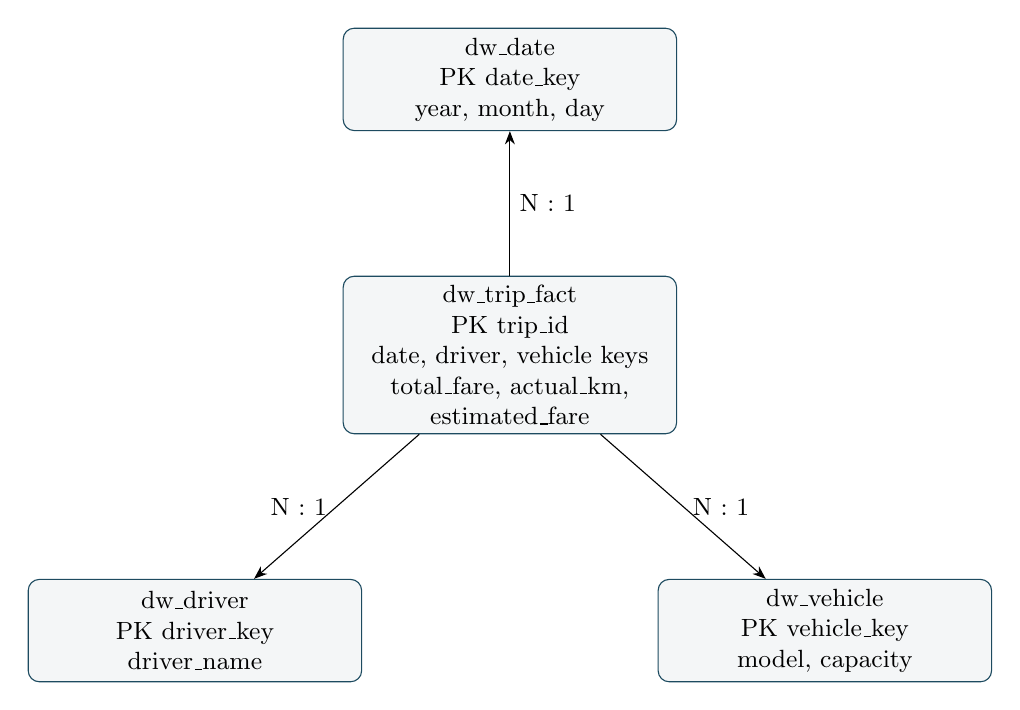
\begin{tikzpicture}[>=Stealth,box/.style={draw=accent,fill=accent!5,rounded corners,align=center,text width=4cm,minimum height=1.3cm,font=\small}]
\node[box](f)at(0,0){dw\_trip\_fact\\PK trip\_id\\date, driver, vehicle keys\\total\_fare, actual\_km, estimated\_fare};
\node[box](d)at(0,3.5){dw\_date\\PK date\_key\\year, month, day};
\node[box](r)at(-4,-3.5){dw\_driver\\PK driver\_key\\driver\_name};
\node[box](v)at(4,-3.5){dw\_vehicle\\PK vehicle\_key\\model, capacity};
\draw[->](f)--node[right,font=\small]{N : 1}(d);\draw[->](f)--node[left,font=\small]{N : 1}(r);\draw[->](f)--node[right,font=\small]{N : 1}(v);
\end{tikzpicture}\end{center}
实际执行的 ROLLUP 按完成年份、月份、车型分组，产生车型明细、月小计、年小计和总计。本数据只覆盖一个月，因此后三层总额恰好相同。分组输出中的 NULL 表示汇总层级，并非维度值缺失；维度来源字段本身不为空。

分析事实表有 130 行，与 CompletedTrip 一致，总费用为 7853.92，与 trip\_\allowbreak{}financials 完全相符。行程编号唯一，并检查可选附加费及评价连接不会放大行数。这类核对能发现一对多连接把金额重复累计的问题。

配套查询还使用 LAG 比较相邻有观测记录日期的费用，并用标量子查询与 HAVING 筛选平均费用高于整体平均的司机。LAG 表示前一个有记录的日期；如果某天没有记录，不能自动理解为前一个自然日。全部结果保存在 TSV 和 JSON 中。

\begin{lstlisting}
SELECT d.calendar_year,d.calendar_month,v.model,
 COUNT(*) AS trips,SUM(f.total_fare) AS gross_fare
FROM dw_trip_fact f
JOIN dw_date d ON d.date_key=f.date_key
JOIN dw_vehicle v ON v.vehicle_key=f.vehicle_key
GROUP BY d.calendar_year,d.calendar_month,v.model WITH ROLLUP;
\end{lstlisting}
\par\begingroup\small\noindent
\begin{tabularx}{\linewidth}{YYYYY}
\toprule
年 & 月 & 车型 & 行程数 & 费用\\\midrule
2026 & 10 & Electric & 39 & 2053.68\\
2026 & 10 & MPV & 45 & 2722.32\\
2026 & 10 & Sedan & 46 & 3077.92\\
2026 & 10 & NULL & 130 & 7853.92\\
2026 & NULL & NULL & 130 & 7853.92\\
NULL & NULL & NULL & 130 & 7853.92\\
\bottomrule
\end{tabularx}
\par\endgroup

\subsection{设计局限与结论}
相对于起始文档，核心改进在于需求、图、关系键和实际行为彼此一致：下单可以早于派车；每个已服务订单能识别实际车辆；终态详情与所有未完成行程明确区分；范式结论有明确依赖依据。

车辆固定归属是控制规模的有意简化，不能推广到司机随时间共享车辆的平台。若需要该场景，应优先引入带时间的分配历史。每单一条双向评价记录适用于一名乘客和一名司机；多次评价、审核和修改历史需要额外结构。

应用角色保护数据库流程完整性，但它是服务级角色，不是按具体客户隔离的数据权限。应用仍需确认登录者是否有权评价某单或查看个人信息。身份认证、逐行访问、加密策略、保留期限和生产监控不属于本数据库演示。

轮班重叠、跨订单司机可用性、派单时保险有效性及取消费用没有自动执行。虽然已存储的数据支持部分检查查询，但不能把保存记录理解为已完成业务规则引擎。费用记录也不证明资金实际支付或结算。

样本小、由程序生成并刻意覆盖边界情况。执行计划只能说明所选访问路径，不能充当性能基准。并发测试仅覆盖两个请求完成同一订单。部署前还需要负载测试、故障恢复、运行权限、更完整的状态变化及代表性数据。

在这些边界内，项目完成了从业务需求、概念和逻辑设计到可执行实现和数据用途讨论的完整过程。分析扩展用于展示 OLTP 与 OLAP 的不同目标，而不替代运营模型。


\appendix
\clearpage
\section{数据字典}
下列定义直接提取自运行数据库的 information\_\allowbreak{}schema，反映实际执行的结构。PRI 表示主键组成部分，UNI 表示唯一索引，MUL 表示非唯一索引列，本身不能证明该列有外键；外键引用对象见关系映射部分。

所有编号由数据加载程序明确提供，不依赖自动编号语法。缺失的可选值使用 SQL NULL；电话号码使用文本类型；金额使用 DECIMAL，避免浮点误差影响费用汇总。

\begingroup\renewcommand{\arraystretch}{1.08}\titlespacing*{\subsection}{0pt}{7pt}{3pt}\subsection*{app\_\allowbreak{}user / 用户}
\par\begingroup\small\noindent
\begin{tabularx}{\linewidth}{p{4.4cm}p{4.0cm}p{1.5cm}X}
\toprule
字段 & SQL 类型 & 可为空 & 键标记\\\midrule
user\_\allowbreak{}id & int & NO & PRI\\
full\_\allowbreak{}name & varchar(80) & NO & —\\
phone & varchar(20) & NO & UNI\\
email & varchar(120) & YES & —\\
birth\_\allowbreak{}date & date & YES & —\\
\bottomrule
\end{tabularx}
\par\endgroup
\subsection*{passenger / 乘客}
\par\begingroup\small\noindent
\begin{tabularx}{\linewidth}{p{4.4cm}p{4.0cm}p{1.5cm}X}
\toprule
字段 & SQL 类型 & 可为空 & 键标记\\\midrule
passenger\_\allowbreak{}id & int & NO & PRI\\
tier & varchar(10) & NO & —\\
\bottomrule
\end{tabularx}
\par\endgroup
\subsection*{driver / 司机}
\par\begingroup\small\noindent
\begin{tabularx}{\linewidth}{p{4.4cm}p{4.0cm}p{1.5cm}X}
\toprule
字段 & SQL 类型 & 可为空 & 键标记\\\midrule
driver\_\allowbreak{}id & int & NO & PRI\\
license\_\allowbreak{}no & varchar(30) & NO & UNI\\
lifetime\_\allowbreak{}km & decimal(12,2) & NO & —\\
\bottomrule
\end{tabularx}
\par\endgroup
\endgroup
\begingroup\renewcommand{\arraystretch}{1.08}\titlespacing*{\subsection}{0pt}{7pt}{3pt}\subsection*{vehicle / 车辆}
\par\begingroup\small\noindent
\begin{tabularx}{\linewidth}{p{4.4cm}p{4.0cm}p{1.5cm}X}
\toprule
字段 & SQL 类型 & 可为空 & 键标记\\\midrule
plate & varchar(12) & NO & PRI\\
driver\_\allowbreak{}id & int & NO & MUL\\
model & varchar(40) & NO & —\\
color & varchar(20) & NO & —\\
capacity & smallint & NO & —\\
\bottomrule
\end{tabularx}
\par\endgroup
\subsection*{insurance\_\allowbreak{}policy / 保险}
\par\begingroup\small\noindent
\begin{tabularx}{\linewidth}{p{4.4cm}p{4.0cm}p{1.5cm}X}
\toprule
字段 & SQL 类型 & 可为空 & 键标记\\\midrule
policy\_\allowbreak{}id & int & NO & PRI\\
plate & varchar(12) & NO & MUL\\
valid\_\allowbreak{}from & date & NO & —\\
valid\_\allowbreak{}to & date & NO & —\\
\bottomrule
\end{tabularx}
\par\endgroup
\subsection*{driver\_\allowbreak{}shift / 轮班}
\par\begingroup\small\noindent
\begin{tabularx}{\linewidth}{p{4.4cm}p{4.0cm}p{1.5cm}X}
\toprule
字段 & SQL 类型 & 可为空 & 键标记\\\midrule
driver\_\allowbreak{}id & int & NO & PRI\\
shift\_\allowbreak{}start & datetime & NO & PRI\\
shift\_\allowbreak{}end & datetime & YES & —\\
\bottomrule
\end{tabularx}
\par\endgroup
\endgroup
\begingroup\renewcommand{\arraystretch}{1.08}\titlespacing*{\subsection}{0pt}{7pt}{3pt}\subsection*{trip / 行程}
\par\begingroup\small\noindent
\begin{tabularx}{\linewidth}{p{4.4cm}p{4.0cm}p{1.5cm}X}
\toprule
字段 & SQL 类型 & 可为空 & 键标记\\\midrule
trip\_\allowbreak{}id & int & NO & PRI\\
passenger\_\allowbreak{}id & int & NO & MUL\\
plate & varchar(12) & YES & MUL\\
requested\_\allowbreak{}at & datetime & NO & —\\
started\_\allowbreak{}at & datetime & YES & —\\
origin\_\allowbreak{}zone & varchar(30) & NO & —\\
destination\_\allowbreak{}zone & varchar(30) & NO & —\\
service\_\allowbreak{}type & varchar(12) & NO & —\\
estimated\_\allowbreak{}km & decimal(8,2) & NO & —\\
estimated\_\allowbreak{}fare & decimal(10,2) & NO & —\\
status & varchar(12) & NO & MUL\\
\bottomrule
\end{tabularx}
\par\endgroup
\endgroup
\begingroup\renewcommand{\arraystretch}{1.08}\titlespacing*{\subsection}{0pt}{7pt}{3pt}\subsection*{completed\_\allowbreak{}trip / 完成行程}
\par\begingroup\small\noindent
\begin{tabularx}{\linewidth}{p{4.4cm}p{4.0cm}p{1.5cm}X}
\toprule
字段 & SQL 类型 & 可为空 & 键标记\\\midrule
trip\_\allowbreak{}id & int & NO & PRI\\
ended\_\allowbreak{}at & datetime & NO & —\\
base\_\allowbreak{}fare & decimal(10,2) & NO & —\\
tip & decimal(10,2) & NO & —\\
actual\_\allowbreak{}km & decimal(8,2) & NO & —\\
\bottomrule
\end{tabularx}
\par\endgroup
\subsection*{cancelled\_\allowbreak{}trip / 取消行程}
\par\begingroup\small\noindent
\begin{tabularx}{\linewidth}{p{4.4cm}p{4.0cm}p{1.5cm}X}
\toprule
字段 & SQL 类型 & 可为空 & 键标记\\\midrule
trip\_\allowbreak{}id & int & NO & PRI\\
cancelled\_\allowbreak{}at & datetime & NO & —\\
reason & varchar(160) & NO & —\\
\bottomrule
\end{tabularx}
\par\endgroup
\subsection*{review / 评价}
\par\begingroup\small\noindent
\begin{tabularx}{\linewidth}{p{4.4cm}p{4.0cm}p{1.5cm}X}
\toprule
字段 & SQL 类型 & 可为空 & 键标记\\\midrule
trip\_\allowbreak{}id & int & NO & PRI\\
passenger\_\allowbreak{}score & smallint & YES & —\\
passenger\_\allowbreak{}comment & varchar(200) & YES & —\\
driver\_\allowbreak{}score & smallint & YES & —\\
driver\_\allowbreak{}comment & varchar(200) & YES & —\\
\bottomrule
\end{tabularx}
\par\endgroup
\subsection*{surcharge / 附加费}
\par\begingroup\small\noindent
\begin{tabularx}{\linewidth}{p{4.4cm}p{4.0cm}p{1.5cm}X}
\toprule
字段 & SQL 类型 & 可为空 & 键标记\\\midrule
trip\_\allowbreak{}id & int & NO & PRI\\
amount & decimal(10,2) & NO & —\\
\bottomrule
\end{tabularx}
\par\endgroup
\endgroup
\clearpage
\section{参考材料与复现说明}
项目说明要求背景和需求、ER/EER 设计、关系设计、数据库实现，以及建库与数据使用讨论。本报告按此流程展开。下表说明已有课件与报告的对应关系。所提供文件中没有 Lecture 1，因此不把未见材料中的内容当作具体要求。

原网约车文档是起始设计。已删除误写的网上商城术语。不把课堂例子推断为额外的实体数量、界面实现或数据仓库必交要求；仓库是范围明确的分析扩展。

\par\begingroup\small\noindent
\begin{tabularx}{\linewidth}{YY}
\toprule
资料 & 应用概念\\\midrule
Group Project Requirements, Fall 2026 & 五个开发环节及深度、可靠性要求\\
LN2 Relational data model & 值域、键、完整性与业务背景\\
LN3 Conceptual model and ER diagrams I & 实体、属性、基数与弱实体\\
LN4 Conceptual model and ER diagrams II & 部分/全部与重叠/互斥特化\\
LN5 Logical design and theory I & 实体、联系和子类到关系的映射\\
LN6 Logical design and theory II & 函数依赖及 1NF、2NF、3NF、BCNF\\
LN7 SQL basic & MySQL DDL、约束及增删改查\\
LN8 SQL basic & NULL、连接、聚合、筛选和子查询\\
LN9 Advanced SQL & 视图、高级查询和事务\\
LN10 Data Warehouse & OLTP/OLAP、星型模型、ROLLUP 和 LAG\\
\bottomrule
\end{tabularx}
\par\endgroup
\subsection*{Implementation references}
\begin{itemize}\small
\item MySQL 8.4 Reference Manual, \emph{CHECK Constraints}: \url{https://dev.mysql.com/doc/refman/8.4/en/create-table-check-constraints.html}.
\item MySQL 8.4 Reference Manual, \emph{Locking Reads}: \url{https://dev.mysql.com/doc/refman/8.4/en/innodb-locking-reads.html}.
\item MySQL 8.4 Reference Manual, \emph{GROUP BY Modifiers}: \url{https://dev.mysql.com/doc/refman/8.4/en/group-by-modifiers.html}.
\end{itemize}
使用独立的 MySQL 8.4 实例，确保没有同名 schema。建库脚本在 ride\_\allowbreak{}hailing 已存在时会报错，不会自动清空已有数据库。按顺序运行结构、过程、生成数据、仓库和角色脚本，再执行验证程序。README 提供完整命令及独立实例说明。

SQL 文件是可执行的依据。create\_\allowbreak{}logic.py 生成过程定义；generate\_\allowbreak{}data.py 重新生成相同数据；run\_\allowbreak{}validation.py 运行检查并导出结果；build\_\allowbreak{}reports.py 读取这些结果和服务器数据字典，生成两个 LaTeX 版本。也可以直接使用交付的 .tex 文件编译 PDF。

成功验证使用 MySQL 8.4.13，数据放在独立临时目录，关闭 TCP 网络监听。受限环境无法正常初始化和连接服务器，因此在该限制之外通过本地 socket 执行。这是运行环境说明，不代表测试未运行；所有报告中的检查均已实际执行。

报告只展示必要的 SQL 和结果以便阅读，同时提供完整脚本、原始查询输出、测试记录和由数据库导出的数据字典，使读者能独立核验设计结论。

\par\begingroup\small\noindent
\begin{tabularx}{\linewidth}{YY}
\toprule
文件或目录 & 用途\\\midrule
report\_\allowbreak{}en.pdf / report\_\allowbreak{}zh.pdf & 英文报告与中文对照版\\
source/report\_\allowbreak{}en.tex / report\_\allowbreak{}zh.tex & 可编辑的 LaTeX 源码\\
sql/01\_\allowbreak{}schema.sql … 07\_\allowbreak{}report\_\allowbreak{}demonstrations.sql & 运营结构、生命周期、数据、仓库、查询及角色\\
scripts/ & 生成、验证、报告编译及运行辅助程序\\
results/validation.json & 32 项测试结果及错误证据\\
results/query\_\allowbreak{}results.json and *.tsv & 实际查询输出，含 EXPLAIN\\
results/report\_\allowbreak{}evidence.json & 表样例及增删改查结果\\
figures/ & 四类图：PDF、SVG、PNG 及可编辑 draw.io\\
results/data\_\allowbreak{}dictionary.tsv & 实际字段元数据\\
README.md & 复现说明与兼容性说明\\
\bottomrule
\end{tabularx}
\par\endgroup

\clearpage
\section{成员职责（草稿）}
本工作表只记录目前已经确认的范围，不是互评分数表，也不替代项目要求提到的独立 Group Project Contribution Form。其余五位成员的职责在本稿中暂未分配，不推测贡献比例。

Lin Shuaiyu已确认负责总体报告主题确定、需求与业务范围分析、ER/EER 概念设计，以及关系映射和规范化等逻辑设计，范围截至具体样例数据准备之前。可能后续承担的数据生成、实现或整合工作，目前不列为已经确认的职责。

\par\begingroup\small\noindent
\begin{tabularx}{\linewidth}{p{2.7cm}p{3cm}X}
\toprule
成员 & 学号 & 已确认范围／占位\\\midrule
Lin Shuaiyu & 226040384 & 主题确定；需求与范围；ER/EER 设计；关系映射与规范化。\\
Cai Ruihe & 226040421 & 待确认：暂留占位，尚未分配。\\
Li Songzi & 226040351 & 待确认：暂留占位，尚未分配。\\
Wen Zhang & 226040373 & 待确认：暂留占位，尚未分配。\\
Zhang Xiujie & 226040424 & 待确认：暂留占位，尚未分配。\\
Jin Conghao & 122090871 & 待确认：暂留占位，尚未分配。\\
\bottomrule
\end{tabularx}
\par\endgroup
\end{document}
